%==============================================================================
% Importando a classe
%==============================================================================
\documentclass{templufla}          


%==============================================================================
% Configuração dos pacotes necessários
%==============================================================================
% Primeiros pacotes (alguns precisam ser importados depois)

% TEXTOS
\usepackage[brazilian]{babel}    % hifenização e títulos em português do Brasil
\usepackage[T1]{fontenc}         % usa fontes postscript com acentos
\usepackage[utf8]{inputenc}      % permite edição direta com acentos

% MATEMÁTICA
\usepackage{amsmath}             % pacote da AMS para Matemática Avançada
\usepackage{amssymb}             % símbolos extras da AMS

% TABELAS
\usepackage{array}               % para mais opções em tabelas
\usepackage{booktabs}            % tabelas geradas por scripts/monografia_tabelas.py

% FIGURAS E GRÁFICOS
\usepackage{xcolor}              % para mais cores
\usepackage{caption}             % para remodelar o formato dos títulos
\usepackage{icomma}              % vírgula decimal sem espaço extra em modo matemático

% O plano gratuito do Overleaf interrompe a compilação em 10 s. Por isso foram removidos os pacotes do
% template que este trabalho não usa (listings, fancyvrb, mathtools, latexsym, longtable, colortbl, multirow,
% multicol, subfigure) e o TikZ: os diagramas de figuras/diagramas/*.pdf são pré-compilados a partir de
% figuras/tikz/*.tex por scripts/compilar_diagramas.py.

%==============================================================================
% O pacote hyperref para referência cruzadas dentro do documento \ref e \autoref

% Setspace precisa estar antes do hyperref para usar a versão atual do abntex.
\usepackage{setspace}

% Definindo cores para os links cruzados
\definecolor{rltred}{rgb}{0.2,0,0}
\definecolor{rltgreen}{rgb}{0,0.2,0}
\definecolor{rltblue}{rgb}{0,0,0.2}


% Importa hyperref
\usepackage[%
hidelinks, % colorlinks=true, | Troque se quiser link com cor
urlcolor=rltblue,       % \href{...}{...} external (URL)
filecolor=rltgreen,     % \href{...} local file
linkcolor=rltred,       % \ref{...} and \pageref{...}
citecolor=rltgreen,%
]{hyperref} % 


%==============================================================================
% Citações/referências no formato ABNT, utilizando o pacote abntex2.
% O pacote já vem na maioria das distribuições (texLive, MikTeX, Overleaf e etc...)
% mas, caso você seja super roots e não use os listados, precisa instalar o abntex2:
% http://abntex.codigolivre.org.br/

% A versão disponível com esse template sofreu algumas alterações para se adaptar ao
% padrão atual, já que a original está desatualizada.
% Para mais informações, vizite o repositório oficial do template.


% abnt-emphasize=bf coloca o título das bibliografias em negrito
% abnt-etal-list=3 limita o número de autores antes de et al. para 3
% abnt-url-package=xurl diz para usar o pacote xurl
\usepackage[alf, abnt-etal-list=3, abnt-url-package=xurl, abnt-emphasize=bf]{abntex2cite}

%==============================================================================
% Ajustando os pacotes importados

% Marcador de trechos pendentes (dados, código ou fontes a preencher). Apague antes de entregar.

\newcommand{\pendente}[1]{\textcolor{red}{\textbf{[PENDENTE: #1]}}}

% Definindo cores para elementos tabulares
\newcolumntype{L}[1]{>{\raggedright\let\newline\\\arraybackslash\hspace{0pt}}m{#1}}
\newcolumntype{C}[1]{>{\centering\let\newline\\\arraybackslash\hspace{0pt}}m{#1}}
\newcolumntype{R}[1]{>{\raggedleft\let\newline\\\arraybackslash\hspace{0pt}}m{#1}}

% Definindo espaçamento vertical de elementos tabulares
\renewcommand{\arraystretch}{1.2}

% Posicionamento de figuras e tabelas mais flexível (UK TeX FAQ, "FAQ-floats"): menos páginas com uma figura
% sozinha e muito espaço em branco
\renewcommand{\topfraction}{0.85}
\renewcommand{\bottomfraction}{0.7}
\renewcommand{\textfraction}{0.15}
\renewcommand{\floatpagefraction}{0.66}
\setcounter{topnumber}{9}
\setcounter{bottomnumber}{9}
\setcounter{totalnumber}{20}

% Carregamento do glossário, listas de siglas, símbolos e etc
\loadglsentries{glossarios/abreviaturas}
\loadglsentries{glossarios/glossario}
\loadglsentries{glossarios/siglas}
\loadglsentries{glossarios/simbolos}

% Especificando hifenizações que por ventura LaTeX não saiba fazer
% Por padrão 99,9% dos termos em português devem ser hifenizados corretamente.
% Adicione aqui palavras precise especificar como hifenizar (ou não hifenizar)
\hyphenation{software am-bien-te coor-de-na-ção FAE-PE TelEduc Williams UFLA Murray Bookchin}

% Adaptando os nomes das seções
% Também pode ser usado para alterar a lingua dos elementos
% (ex Figura para Figure, caso seu texto esteja em inglês).
\addto\captionsbrazilian{
	\renewcommand{\chaptername}{Seção}
	\renewcommand{\subsectionname}{Seção}
	\renewcommand{\subsubsectionname}{Seção}
	%\renewcommand{\figurename}{Figure}
}
\addto\extrasbrazilian{
	\renewcommand{\chapterautorefname}{Seção}
	\renewcommand{\subsectionautorefname}{Seção}
	\renewcommand{\subsubsectionautorefname}{Seção}
	%\renewcommand{\figureautorefname}{Figure}
}


%==============================================================================
% Dados da monografia, capa: autor, titulo, banca, etc... - SUBSTITUA DE ACORDO
%==============================================================================
% Dados para o arquivo PDF (metadados)
\hypersetup{%
% Titulo
pdftitle={Estimação do Ângulo de Deriva em Veículos Inteligentes utilizando Programação Genética Multigene},
% Autor
pdfauthor={Alexsander Miguel do Sacramento},
% Descrição
pdfsubject={Trabalho de conclusão de curso, Engenharia de Controle e Automação, UFLA},
% Palavras-Chave
pdfkeywords={ângulo de deriva; programação genética multigene; sensor virtual; veículos inteligentes}
}
	
%==============================================================================
% Informações básicas

% Nome da(s)/do(s) autora(s)/autor(es)
\author{Alexsander Miguel do Sacramento}

% Título do trabalho, em lígua vernácula
\title{Estimação do Ângulo de Deriva em Veículos Inteligentes utilizando Programação Genética Multigene}


% Título do trabalho, em inglês
\engtitle{Sideslip Angle Estimation in Intelligent Vehicles using Multigene Genetic Programming}



% Data de publicação
\date{2026}

% Tipo do Documento
\tipo{Trabalho de conclusão de curso apresentado à Universidade Federal de Lavras, como parte das exigências do Curso de Engenharia de Controle e Automação, para a obtenção do título de Bacharel.}


% Orientador/orientadora
% Altere o comando para os diferentes gêneros
\orientador{Prof. Dr. Bruno Henrique Groenner Barbosa}
%\orientadora{Profa. DSc. Maria Orientadora}

% Coorientador/coorientadora
% Altere o comando para os diferentes gêneros
% Comente se não houver.
%\coorientador{Prof. DSc. José Orientador}

% Local
\local{Lavras -- MG}

%==============================================================================
% Informações da banca

% Membros da banca. Até quatro membros. 
% Deve ser {nome}{instituição}.
% Comente os últimos se a banca tiver menos membros.
\bancaum{A DEFINIR}{UFLA}
\bancadois{A DEFINIR}{UFLA}
\bancatres{A DEFINIR}{A DEFINIR}
%\bancaquatro{A DEFINIR}{A DEFINIR}

% Data da defesa
\defesa{A DEFINIR}

%==============================================================================
% Dados para Ficha catalográfica, gerada pelo sistema da Biblioteca da UFLA
% http://www.biblioteca.ufla.br/FichaCatalografica/
% dados para ficha catalográfica

% Texto acima da ficha
\preparofichacat{Ficha catalográfica elaborada pela Coordenadoria de Processos Técnicos da Biblioteca Universitária da UFLA, com dados informados pelo(a) próprio(a) autor(a).}

% Primeiro autor - como na primeira linha da ficha catalográfica
%\fcautor{Sacramento, Alexsander Miguel do} % ficha omitida: não obrigatória na graduação (manual UFLA, 6. ed., §3.1.2.1.2)

% Autores, separados por vírgula - na ficha catalográfica, no formato que
% vem após o título e a barra ("/")
\fcautores{Alexsander Miguel do Sacramento}

% Numero de páginas,
% Caso o valor seja diferente do calculado, basta descomentar e adicionar.
%\fcnpaginas{777}

% Caso trabalho seja ilustrado (figuras, gráficos, tabelas, etc.).
% Caso não seja ilustrado, basta comentá-lo
\fcilustrado{il.}

% Dados da edição para a ficha 
%\fcedicao{}

% Tipo do trabalho (tese, dissertação, etc.), de acordo com sistema
% de geração de ficha catalográfica
\fctipo{TCC (graduação)}

% Ano da defesa, só precisa informar se for diferente do ano da publicação
% se forem iguais, comente a linha a seguir
%\fcdatadefesa{2025}

% Preencher aqui com os dados de catalogação gerados pelo sistema
\fccatalogacao{A DEFINIR}
\fcclasi{A DEFINIR}

%==============================================================================
% Se vc já defendeu e tem o arquivo escaneado da folha de rosto, 
% descomente e altere o nome do arquivo
%\folhaAprovacaoAssinada{folharosto}


%==============================================================================
% O documento em si
%==============================================================================
\begin{document}

%==============================================================================
%Elementos pré-textuais

% Cria capa, folha de rosto, folha de aprovação e ficha
\maketitle


% Agradecimentos: opcionais (manual UFLA, 6. ed., §3.1.2.1.6); reinserir \thanks{...} quando houver texto (GOALS 6.7.2)


% Resumo e palavras-chave
% As palavras-chave PRECISAM vir primeiro
\palchaves{ângulo de deriva; programação genética multigene; sensor virtual; veículos inteligentes; identificação de sistemas.}
\resumo{%
O ângulo de deriva é uma variável central do controle de estabilidade de veículos, mas sua medição direta exige sensores de alto custo. Este trabalho investiga sua estimação por um sensor virtual baseado em Programação Genética Multigene (MGGP), dando continuidade a um modelo desenvolvido em Iniciação Científica que estima as velocidades longitudinal e lateral a partir das acelerações longitudinal e lateral, das velocidades das rodas e da taxa de guinada. A pergunta central é se o ângulo de deriva é mais bem estimado como terceira saída do modelo multivariável ou calculado a partir das velocidades estimadas, por $\operatorname{atan2}(\hat v_y, \hat v_x)$. Com dados experimentais de um veículo instrumentado e a melhor configuração de hiperparâmetros da pesquisa anterior, foram treinados 30 modelos com duas saídas e 28 aprovados com três saídas (dois foram reprovados na validação). Os modelos foram avaliados em simulação livre em três ensaios não usados no treinamento, segundo um plano de análise definido antes do processamento dos resultados finais. Em dois dos três ensaios não houve diferença significativa entre as abordagens. No terceiro, os modelos com três saídas reduziram a mediana do erro quadrático médio do ângulo de deriva de 1,74° para 1,10°, com efeito grande, mas nesse ensaio, como nos demais de teste, a velocidade lateral de referência está deslocada em cerca de 0,3 m/s em relação ao valor implícito no ângulo de deriva bruto. Esse ganho não resiste à correção do deslocamento: com a referência corrigida, os modelos com duas saídas erram menos nos três ensaios. A terceira saída piorou significativamente a velocidade longitudinal em dois ensaios e aumentou em cerca de 70\% o custo de treinamento. A saída evoluída e o ângulo calculado a partir das velocidades do mesmo modelo foram praticamente equivalentes. Conclui-se que não há evidência robusta de que a terceira saída melhore o ângulo de deriva: o ganho foi observado em um único ensaio, depende da referência adotada e vem acompanhado de custo na velocidade longitudinal e no tempo de treinamento. Quando as velocidades também são utilizadas, o cálculo a partir delas é preferível.
}

% Abstract e keywords
% As keywords PRECISAM vir primeiro
\keywords{sideslip angle; multigene genetic programming; virtual sensor; intelligent vehicles; system identification.}
\abstract{%
The sideslip angle is a central variable in vehicle stability control, but measuring it directly requires expensive sensors. This work investigates its estimation by a virtual sensor based on Multigene Genetic Programming (MGGP), continuing a model developed in an undergraduate research project that estimates the longitudinal and lateral velocities from the longitudinal and lateral accelerations, the wheel speeds and the yaw rate. The central question is whether the sideslip angle is better estimated as a third output of the multivariable model or computed from the estimated velocities, as $\operatorname{atan2}(\hat v_y, \hat v_x)$. Using experimental data from an instrumented vehicle and the best hyperparameter configuration of the previous research, 30 two-output models and 28 approved three-output models were trained (two were rejected in validation). They were evaluated in free-run simulation on three tests not used for training, following a statistical analysis plan defined before the final results were processed. In two of the three test runs there was no significant difference between the approaches. In the third, the three-output models reduced the median root mean square error of the sideslip angle from 1.74° to 1.10°, with a large effect size; however, in this run, as in the other test runs, the reference lateral velocity is offset by about 0.3 m/s from the value implied by the raw sideslip angle. This gain does not survive correcting the offset: with the corrected reference, the two-output models have lower error in all three test runs. The third output significantly worsened the longitudinal velocity in two test runs and increased the training cost by about 70\%. The evolved output and the angle computed from the same model's velocities were practically equivalent. It is concluded that there is no robust evidence that the third output improves the sideslip angle: the gain was observed in a single run, depends on the adopted reference, and comes with a cost in longitudinal velocity and training time. When the velocities are also used, computing the angle from them is preferable.
}


% Listas gerais
% Comente para remover.
% Listas de figuras e de tabelas omitidas (opcionais, manual §3.1.2.1.11–12; GOALS 6 reserva R1)
%\listofilustracoes % Lista de Ilustrações
%\listofgraficos	% Lista de Gráficos
%\listofquadros		% Lista de Quadros
%\listofexemplos    % Lista de Exemplos
%\listofteoremas    % Lista de Teoremas
%\listofabreviaturas % Lista de Abreviaturas
% Lista de abreviaturas e siglas (todas as entradas de glossarios/siglas.tex)
\glsaddall
\listofsiglas

% Sumário
\tableofcontents
\clearpage

%==============================================================================
% Elementos textuais

% Começa a mostrar a numeração
\pagestyle{ufla}


% Incluindo as seções
% É recomendado que as seções sejam organizadas em arquivos separados
% e incluídas no documento com o comando \include
\chapter{INTRODUÇÃO}\label{sec:introducao}

A estimação precisa das velocidades longitudinais e laterais desempenha papel importante em termos de segurança, estabilidade e eficiência operacional. Essas velocidades são fundamentais para o controle de veículos, especialmente em condições como curvas acentuadas, mudanças repentinas de direção e situações de emergência. Além disso, a determinação dessas velocidades permite calcular o ângulo de deriva, um parâmetro utilizado para avaliar a estabilidade direcional, prevenir acidentes e analisar o desempenho dinâmico \cite{wang2023}.

Métodos baseados em modelos físicos enfrentam obstáculos decorrentes da necessidade de uma modelagem detalhada do comportamento do veículo, levando em conta forças como o atrito dos pneus e os efeitos aerodinâmicos. Essa abordagem resulta em equações matemáticas complexas e não lineares, aplicadas em cenários dinâmicos \cite{singh2018}. A complexidade se eleva quando se considera condições como variações de terreno ou mudanças climáticas, situações em que os métodos tradicionais podem apresentar limitações para acompanhar a dinâmica do ambiente \cite{viehweger2020}.

Algoritmos de Inteligência Artificial (IA), como a Programação Genética Multigene (MGGP), destacam-se por evoluir múltiplos genes que se combinam para gerar expressões simbólicas capazes de modelar relações não lineares entre leituras de sensores e as velocidades longitudinal e lateral, sem exigir um modelo físico explícito \cite{mota2022}. Além disso, sensores virtuais baseados em dados podem utilizar sensores convencionais, como acelerômetros e giroscópios, reduzindo custos de implementação \cite{kong2022}. Estudos recentes indicam que ferramentas de IA podem atingir resultados comparáveis aos obtidos com sensores de custo elevado, posicionando-se como uma alternativa para veículos inteligentes e comerciais \cite{jin2021}.

Ao contrário de modelos baseados em estruturas de tipo caixa-preta, o MGGP utiliza a evolução simbólica para derivar expressões matemáticas que, além de capturarem relações não lineares entre os sinais de sensores --- como acelerômetros e giroscópios --- e as velocidades $v_x$ e $v_y$, mantêm um nível de interpretabilidade para a engenharia de controle \cite{olson2010, castro2023}.

Entre as grandezas que um sensor virtual pode fornecer, o ângulo de deriva ($\beta$) ocupa posição particular. Ele descreve a diferença entre a direção para a qual o veículo aponta e a direção em que de fato se desloca, e é uma das variáveis centrais dos sistemas de controle de estabilidade. Sua medição direta, contudo, exige sensores ópticos ou sistemas de posicionamento global e de navegação inercial (GPS/INS, do inglês \textit{Global Positioning System} e \textit{Inertial Navigation System}) de alto custo, o que motiva a sua estimação a partir de sensores embarcados convencionais \cite{chindamo2018, liu2018}.

Na Iniciação Científica (IC) que antecedeu este trabalho, foi desenvolvido um sensor virtual MGGP com cinco entradas e duas saídas, que estima simultaneamente $v_x$ e $v_y$. A partir dessas estimativas, o ângulo de deriva pode ser obtido diretamente por $\hat\beta = \operatorname{atan2}(\hat v_y, \hat v_x)$. Surge, então, a pergunta que motiva este Trabalho de Conclusão de Curso (TCC): estimar $\beta$ como uma terceira saída do próprio modelo de múltiplas entradas e múltiplas saídas (MIMO, do inglês \textit{Multiple-Input Multiple-Output}) --- de modo que o algoritmo evolutivo o considere durante o treinamento --- produz um ângulo de deriva mais preciso do que calculá-lo depois, a partir das velocidades estimadas? E essa terceira saída altera a qualidade das estimativas de $v_x$ e $v_y$? Como o MGGP ajusta todas as saídas com uma única função de aptidão e realimenta as estimativas de todas elas nas demais, a resposta não é evidente \emph{a priori}, e precisa ser medida.

\section{Objetivos}

O objetivo geral deste trabalho é estimar o ângulo de deriva de um veículo por meio de um sensor virtual simbólico baseado em Programação Genética Multigene, dando continuidade ao modelo desenvolvido na IC, e avaliar se a inclusão de $\beta$ como terceira saída do modelo MIMO melhora essa estimação em relação ao ângulo calculado a partir das velocidades estimadas.

Os objetivos específicos são:

\begin{alineas}
    \item comparar, em pistas não utilizadas no treinamento, o erro de $\beta$ obtido pela terceira saída evoluída de modelos com cinco entradas e três saídas (5×3) com o erro de $\beta$ pós-calculado a partir de modelos com cinco entradas e duas saídas (5×2);
    \item verificar se a terceira saída altera a qualidade das estimativas de $v_x$ e $v_y$ em relação aos modelos 5×2;
    \item comparar, dentro de um mesmo modelo 5×3, a saída evoluída de $\beta$ com o ângulo calculado a partir das velocidades que o próprio modelo estima;
    \item situar esses resultados em relação a um estimador cinemático de $\beta$ e aos modelos de referência da IC, e interpretar fisicamente as equações obtidas para $\beta$.
\end{alineas}

\section{Relação com a Iniciação Científica}

Este TCC reaproveita da IC a base de dados experimental, a biblioteca MGGP em Python, as entradas do sensor virtual e a configuração de hiperparâmetros que produziu o melhor modelo daquela pesquisa. Na IC, uma busca sistemática de 147 configurações estruturais --- sete valores de número de termos, sete de profundidade máxima das árvores e três janelas de atraso --- identificou como melhor configuração a de atrasos $[1, 2, 5, 10, 25, 50]$, sete termos por saída e profundidade máxima seis (denominada T48), com raiz do erro quadrático médio (RMSE, do inglês \textit{Root Mean Square Error}) média de 0,2121~m/s nas velocidades. A IC mostrou, ainda, que as equações obtidas recuperam a forma discreta das equações cinemáticas do modelo de bicicleta. A \autoref{fig:evolucao_ic} resume aquela busca: com um único atraso, muitas configurações divergiram em simulação livre, enquanto as janelas de atraso mais longas estabilizaram os modelos.

\begin{figure}[htbp]
    \centering
    \caption{RMSE médio dos modelos de cada treinamento da busca realizada na IC, por janela de atrasos.}
    \label{fig:evolucao_ic}
    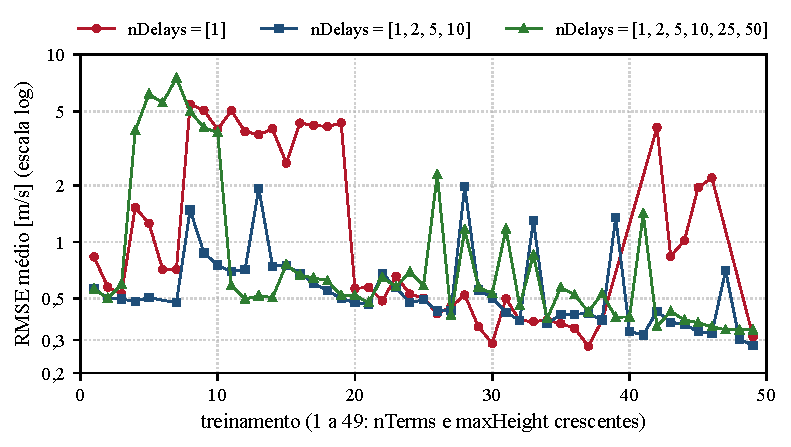
\includegraphics[width=\textwidth]{figuras/evolucao_ic.pdf}
    \fonte{Elaboração própria com dados da IC.}
\end{figure} Neste trabalho, essa configuração é mantida fixa, de modo que qualquer diferença observada entre os modelos 5×2 e 5×3 possa ser atribuída à terceira saída, e não a uma mudança de hiperparâmetros.
\chapter{REFERENCIAL TEÓRICO}\label{sec:referencial}

Esta seção apresenta o modelo de bicicleta, o ângulo de deriva e os métodos para estimá-lo, e os fundamentos de aprendizado supervisionado, programação genética e MGGP em que o trabalho se apoia.

\section{Modelagem veicular e modelo de bicicleta}\label{sec:modelagem_veiculos}

No âmbito deste trabalho, adota-se o modelo de bicicleta, que simplifica o veículo considerando apenas dois pontos de contato com o solo: um no eixo dianteiro e outro no eixo traseiro. O Centro de Gravidade (CG), situado entre esses dois eixos, é tomado como o ponto de referência para a modelagem cinemática. Esse modelo é utilizado devido à sua formulação matemática e capacidade de capturar o comportamento dinâmico do veículo no plano horizontal \cite{viehweger2020}.

A modelagem considera que o veículo pode se mover longitudinalmente ($v_x$) e lateralmente ($v_y$) em relação ao CG, ao mesmo tempo em que realiza rotações em torno de seu eixo vertical, uma grandeza caracterizada pela taxa de guinada ($\dot{\psi}$). Em momentos em que ocorre o esterçamento das rodas dianteiras (ângulo $\delta$) a fim de deslocar o veículo lateralmente, surgem os ângulos de deslizamento da roda dianteira ($\alpha_f$) e da roda traseira ($\alpha_r$), bem como o ângulo de deslizamento lateral do veículo, também denominado ângulo de deriva ($\beta$) \cite{rajamani2012}.

A velocidade longitudinal está associada ao deslocamento na direção do eixo longitudinal do veículo. A variação da velocidade longitudinal ($\dot{v}_x$), expressa pela \autoref{eq:velocidade_longitudinal}, depende da aceleração medida nessa direção e do efeito rotacional combinado à velocidade lateral \cite{jiang2019}:
\begin{equation}
    \dot{v}_x = a_x + \dot{\psi} v_y.
    \label{eq:velocidade_longitudinal}
\end{equation}

A velocidade lateral representa o desvio perpendicular ao eixo longitudinal, sendo resultante de manobras de esterçamento ou forças de perturbação lateral. A variação da velocidade lateral ($\dot{v}_y$), detalhada na \autoref{eq:velocidade_lateral}, relaciona a aceleração lateral à interação existente entre a rotação do veículo e sua velocidade longitudinal \cite{jiang2019}:
\begin{equation}
    \dot{v}_y = a_y - \dot{\psi} v_x.
    \label{eq:velocidade_lateral}
\end{equation}

Na \autoref{fig:modelo_bicicleta}, apresenta-se a representação do modelo de bicicleta, cuja estrutura serviu de base geométrica e cinemática para a modelagem proposta neste trabalho.

\begin{figure}[htbp]
    \centering
    \caption{Modelo de bicicleta para a cinemática veicular, com o ângulo de deriva $\beta$ entre o vetor velocidade $V$ no CG e o eixo longitudinal.}
    \label{fig:modelo_bicicleta}
    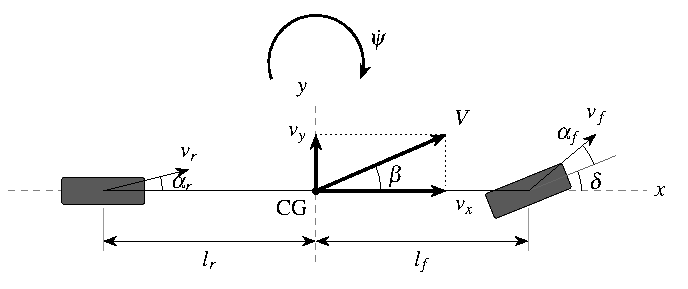
\includegraphics[width=0.85\textwidth]{figuras/diagramas/modelo_bicicleta.pdf}
    \fonte{Elaboração própria, adaptado de \citeonline{rajamani2012}.}
\end{figure}

\section{Ângulo de deriva}\label{sec:angulo_deriva}

O ângulo de deriva é o ângulo entre o vetor velocidade do veículo no CG e o seu eixo longitudinal (\autoref{fig:modelo_bicicleta}). Em função das componentes da velocidade, ele é definido por
\begin{equation}
    \beta = \operatorname{atan2}(v_y, v_x) \approx \frac{v_y}{v_x},
    \label{eq:beta}
\end{equation}
em que a aproximação vale para ângulos pequenos e $v_x > 0$, condição típica da condução normal, na qual $\beta$ raramente ultrapassa alguns graus \cite{rajamani2012}.

Derivando a aproximação da \autoref{eq:beta} no tempo e substituindo as Equações \ref{eq:velocidade_longitudinal} e \ref{eq:velocidade_lateral}, desprezando-se os termos de segunda ordem em $\beta$ e a variação de $v_x$, obtém-se a relação cinemática
\begin{equation}
    \dot{\beta} \approx \frac{a_y}{v_x} - \dot{\psi},
    \label{eq:beta_cinematica}
\end{equation}
que relaciona a evolução do ângulo de deriva a duas grandezas medidas por uma unidade inercial ($a_y$ e $\dot\psi$) e à velocidade longitudinal. A \autoref{eq:beta_cinematica} não depende de parâmetros do pneu nem do veículo, mas exige integração: qualquer viés em $a_y$ ou $\dot\psi$ se acumula ao longo do tempo, e o termo $a_y/v_x$ torna-se mal condicionado em baixa velocidade. Pelo mesmo motivo, o cálculo de $\beta$ por $\operatorname{atan2}(\hat v_y, \hat v_x)$ amplifica o erro de $\hat v_y$ quando $v_x$ é pequeno: um erro $\varepsilon$ em $v_y$ produz um erro aproximado de $\varepsilon / v_x$ em $\beta$.

O ângulo de deriva é uma das variáveis centrais do controle de estabilidade veicular. Valores elevados de $\beta$ indicam que o veículo está próximo do limite de aderência dos pneus e que sua resposta ao volante deixa de ser previsível; por isso, sistemas de controle de estabilidade procuram manter $\beta$ dentro de limites seguros. Como sensores capazes de medir $\beta$ diretamente --- sensores ópticos de velocidade ou sistemas GPS/INS de alta precisão --- têm custo elevado para veículos de série, $\beta$ é, em geral, estimado a partir dos sensores convencionais do veículo \cite{chindamo2018}.

\section{Métodos de estimação do ângulo de deriva}\label{sec:metodos_estimacao}

A literatura organiza os estimadores de ângulo de deriva em três famílias principais \cite{chindamo2018, liu2018}.

Os métodos baseados em modelo cinemático usam apenas relações geométricas e cinemáticas, como a \autoref{eq:beta_cinematica}, alimentadas por acelerômetros, giroscópios e velocidades das rodas. Sua vantagem é a independência de parâmetros do veículo e do pneu; sua desvantagem é a sensibilidade a vieses e ruídos dos sensores, que, integrados, fazem a estimativa derivar ao longo do tempo. Por isso, costumam ser combinados com alguma forma de correção, como medidas de GPS \cite{liu2018}.

Os métodos baseados em modelo dinâmico descrevem as forças laterais nos pneus e usam observadores --- filtros de Kalman e suas variantes, observadores de modos deslizantes, observadores não lineares --- para estimar $\beta$. São precisos dentro da faixa de validade do modelo, mas dependem de parâmetros como a rigidez lateral dos pneus e o coeficiente de atrito com o pavimento, que variam com a carga, o desgaste e a condição da pista \cite{puscul2024}.

Os métodos orientados a dados aprendem a relação entre as medições disponíveis e $\beta$ a partir de ensaios de referência, frequentemente com redes neurais. Dispensam modelos explícitos, mas, em geral, produzem modelos do tipo caixa-preta, de difícil interpretação e certificação \cite{chindamo2018}. A Programação Genética Multigene ocupa uma posição intermediária: é orientada a dados, mas produz equações simbólicas que podem ser inspecionadas e comparadas com a física do problema, como fez a IC para as velocidades. Este trabalho investiga se essa abordagem pode fornecer o ângulo de deriva diretamente, como saída do modelo.

\section{Aprendizado supervisionado e programação genética}

O aprendizado de máquina (\textit{Machine Learning}), uma das subáreas da IA, capacita sistemas computacionais a alterar seu desempenho a partir de dados \cite{filho2024}. No aprendizado supervisionado, paradigma adotado neste trabalho, o modelo é treinado com dados rotulados, em que cada entrada está associada a uma saída conhecida, e deve generalizar essa relação para dados inéditos \cite{pecht2021}. Essa abordagem viabiliza sensores virtuais, que estimam estados dinâmicos do veículo a partir das leituras de sensores convencionais \cite{muhammad2021}.

A Computação Evolutiva (CE) reúne métodos de busca e otimização inspirados na seleção natural: populações de soluções candidatas são submetidas, iterativamente, a operações análogas à reprodução, ao cruzamento (\textit{crossover}) e à mutação, de modo a obter indivíduos cada vez mais aptos a resolver o problema \cite{antunes2012}. Nos Algoritmos Genéticos (AG), formalizados por John Holland na década de 1970, o ciclo segue a \autoref{fig:fluxograma_ag}: gera-se uma população inicial aleatória; calcula-se a aptidão (\textit{fitness}) de cada indivíduo --- neste trabalho, o RMSE; selecionam-se os genitores, por roleta ou torneio; aplicam-se o cruzamento e a mutação, que mantém a diversidade genética; e a nova população substitui a anterior até que se atinja um critério de parada, como o número máximo de gerações. O elitismo impede que as melhores soluções encontradas se percam ao longo das gerações \cite{linder2012}.

\begin{figure}[htbp]
    \centering
    \caption{Fluxograma de execução de um algoritmo genético clássico.}
    \label{fig:fluxograma_ag}
    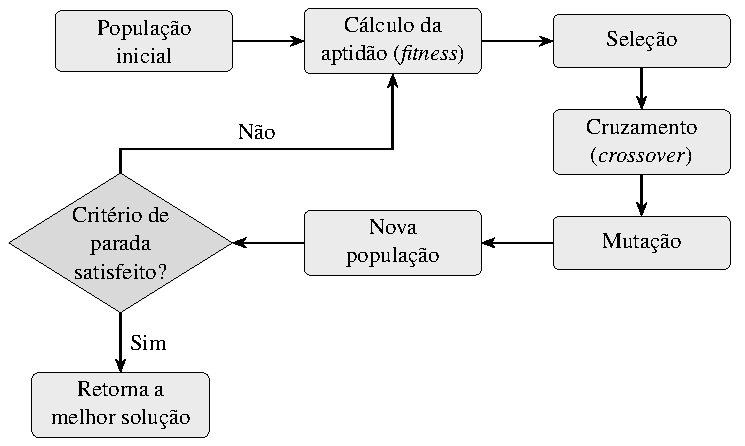
\includegraphics[width=0.7\textwidth]{figuras/diagramas/fluxograma_ag.pdf}
    \fonte{Elaboração própria, adaptado de \citeonline{linder2012}.}
\end{figure}

Na Programação Genética (PG), cada indivíduo é uma árvore sintática: os nós internos contêm funções ou operadores matemáticos, como adição, subtração e multiplicação, e as folhas contêm variáveis de entrada ou constantes. Diferentemente dos AG, que evoluem cromossomos numéricos de tamanho fixo, a PG evolui a própria estrutura do modelo, sem que o projetista precise definir previamente a sua forma \cite{pereda2020}. O cruzamento troca subárvores entre dois genitores, e a mutação substitui um ramo por uma nova subárvore aleatória, o que preserva a diversidade e reduz a convergência prematura \cite{willis1997}. Para limitar o crescimento excessivo das equações (\textit{bloat}), impõe-se uma profundidade máxima às árvores (\textit{maxHeight}); a seleção por torneio e o elitismo completam o processo \cite{koza2009}.

\section{Programação genética multigene e modelos NARX MIMO}\label{sec:mggp}

O MGGP surgiu para separar a busca heurística pela estrutura simbólica de um modelo não linear do ajuste numérico de seus coeficientes. Em vez de evoluir uma única árvore sintática, característica da PG, cada indivíduo no MGGP é formado por um conjunto de genes. Cada gene é representado por uma árvore matemática independente que combina variáveis de entrada e seus respectivos atrasos temporais por meio de operadores simbólicos.

Em cada geração, monta-se uma matriz de regressores que contém, em cada coluna, a avaliação da saída de um desses genes para as amostras do conjunto de treinamento. Em seguida, ajustam-se os coeficientes de ponderação ($\theta$) por meio do Método dos Mínimos Quadrados Ordinários (MQO), de modo que a combinação linear dos genes minimize o erro entre a saída do sistema e a predição. Esse procedimento atua na superfície de aptidão (\textit{fitness landscape}), pois o ajuste dos parâmetros lineares ($\theta$) é delegado a métodos de regressão, enquanto a evolução genética concentra-se em determinar quais genes devem compor o modelo \cite{pandey2015a, pereda2020}.

Os operadores genéticos no MGGP incluem o \textit{crossover} de alto nível, que permuta árvores completas (genes) entre os indivíduos progenitores, e o \textit{crossover} de baixo nível, que insere fragmentos de um progenitor dentro da árvore de outro. Adicionalmente, a mutação pode substituir um gene por uma nova árvore gerada aleatoriamente ou alterar uma subárvore interna, preservando parte da estrutura original \cite{koza2009, willis1997}.

Em problemas de identificação de sistemas dinâmicos, o MGGP é empregado na forma de modelos autorregressivos não lineares com entradas exógenas (NARX, do inglês \textit{Nonlinear AutoRegressive with eXogenous inputs}), em que a saída no instante $k$ depende de valores passados das entradas e das próprias saídas. Na arquitetura MIMO utilizada neste trabalho, cada indivíduo possui um conjunto próprio de genes para cada saída, e os valores atrasados de \emph{todas} as saídas estão disponíveis como terminais para \emph{todas} as árvores. Para uma saída $j$, o modelo assume a forma
\begin{equation}
    \hat y_j[k] = \theta_{j,0} + \sum_{i=1}^{n_T} \theta_{j,i}\, g_{j,i}\big(\mathbf{u}[k-d], \hat{\mathbf{y}}[k-d]\big),
    \label{eq:mggp_mimo}
\end{equation}
em que $n_T$ é o número de termos (genes) por saída, $g_{j,i}$ é o gene $i$ da saída $j$, e $d$ percorre o conjunto de atrasos permitidos. A \autoref{fig:individuo_mggp} ilustra um indivíduo com três saídas --- $\hat v_x$, $\hat v_y$ e $\hat\beta$ --- como os avaliados neste trabalho. Uma consequência importante dessa estrutura é que, quando $\beta$ é incluído como terceira saída, sua estimativa passa a poder ser usada pelas equações de $v_x$ e $v_y$, e vice-versa.

\begin{figure}[htbp]
    \centering
    \caption{Estrutura de um indivíduo MGGP NARX MIMO com três saídas. Cada saída é uma combinação linear de genes; as saídas atrasadas realimentam todas as árvores.}
    \label{fig:individuo_mggp}
    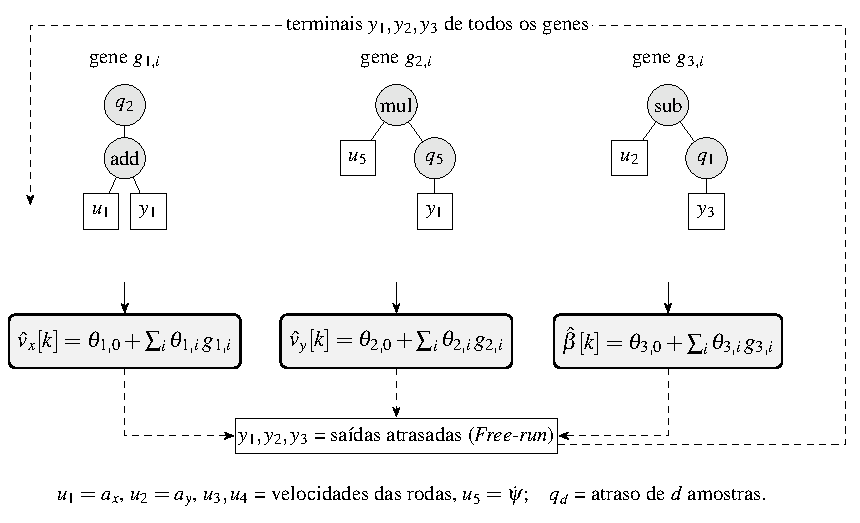
\includegraphics[width=\textwidth]{figuras/diagramas/individuo_mggp.pdf}
    \fonte{Elaboração própria.}
\end{figure}

Na biblioteca utilizada, a aptidão de um indivíduo MIMO é a média simples dos RMSE das saídas, sem normalização --- característica que se torna relevante quando as saídas têm escalas muito diferentes, como discutido na \autoref{sec:metodos}.

Aplicações em sistemas veiculares indicam que essa técnica pode ser utilizada para a construção de sensores virtuais, atendendo aos requisitos de análise na automação \cite{pandey2015a, mota2022, kaneko2022}.

\section{Regimes de simulação}\label{sec:regimes}

Em problemas de identificação de sistemas dinâmicos, adotam-se diferentes regimes de simulação e validação \cite{pandey2015a, kaneko2022}:

\begin{alineas}
    \item predição um passo à frente (\textit{one-step-ahead}): emprega os valores reais defasados do sistema para calcular a próxima predição, fornecendo resultados para análise inicial;
    \item simulação livre (\textit{free-run}): o modelo realimenta suas próprias predições passadas para gerar a sequência futura, evidenciando o comportamento do erro dinâmico ao longo do tempo. No caso MIMO, todas as saídas estimadas são realimentadas;
    \item tiros múltiplos (\textit{multi-shooting}): divide a série temporal em blocos de tamanho $K$, simulando livremente cada bloco e, ao final de cada intervalo, reinicia a predição com o valor real.
\end{alineas}

A simulação livre é o regime que corresponde à operação real de um sensor virtual, que não dispõe da medição da grandeza que estima; por isso, é o regime adotado em toda a avaliação deste trabalho \cite{castro2021}.

\chapter{MATERIAL E MÉTODOS}\label{sec:metodos}

Esta seção descreve a base de dados, a definição do ângulo de deriva de referência, a configuração do MGGP, o desenho experimental, o protocolo de treinamento e o plano de análise estatística.

\section{Base de dados}\label{sec:base_dados}

A base de dados, a mesma utilizada na IC, resulta de uma parceria com a Universidade de Jilin, na China. Os ensaios foram realizados com um veículo instrumentado, no qual um sistema GPS/INS, com a unidade inercial próxima ao centro de massa, fornece a referência das velocidades; o veículo dispõe ainda de transdutores de força e de sensores de pneus inteligentes, não utilizados neste estudo.

A base de dados é composta por cinco ensaios, denominados Wang 2.1, Wang 2.2, Wang 3.1, Wang 8.1 e Wang 3.2, realizados em condições de direção aleatórias (\textit{Random Driving Conditions}) e amostrados a 200~Hz. Cinco variáveis são utilizadas como entradas dos modelos:

\begin{alineas}
    \item aceleração longitudinal, $a_x$ (m/s²);
    \item aceleração lateral, $a_y$ (m/s²);
    \item velocidade angular da roda dianteira, $\omega_f$ (rad/s);
    \item velocidade angular da roda traseira, $\omega_r$ (rad/s);
    \item taxa de guinada, $\dot\psi$ (rad/s).
\end{alineas}

As velocidades longitudinal ($v_x$) e lateral ($v_y$), em m/s, medidas pelo sistema GPS/INS, são as saídas de referência. Na notação da biblioteca, as entradas são $u_1$ a $u_5$, na ordem acima, e as saídas são $y_1 = v_x$, $y_2 = v_y$ e, nos modelos com três saídas, $y_3 = \beta$. As velocidades das rodas são velocidades angulares; nos dados, $v_x$ é aproximadamente proporcional à velocidade da roda traseira, com fator de 0,2988~m/rad (ajustado por mínimos quadrados no ensaio Wang 2.1), compatível com o raio efetivo do pneu.

O comportamento temporal das variáveis do ensaio de treinamento é exibido na \autoref{fig:sinais_wang21}, e a \autoref{tab:pistas} resume o papel de cada ensaio no experimento. O ensaio Wang 2.1 é usado no treinamento; o Wang 2.2, na aprovação dos modelos (\autoref{sec:protocolo}); e os ensaios Wang 3.1, Wang 8.1 e Wang 3.2 não participam de nenhuma decisão de treinamento deste trabalho e constituem as pistas de teste. Ressalta-se, porém, que a configuração T48, herdada da IC, foi escolhida naquela pesquisa observando o desempenho nas pistas Wang 2.1 a 8.1. Assim, a Wang 3.2, que não havia sido utilizada na IC, é a única pista de teste totalmente independente da escolha dos hiperparâmetros.

\begin{figure}[htbp]
    \centering
    \caption{Variáveis do ensaio de treinamento (Wang 2.1): aceleração longitudinal (a), aceleração lateral (b), velocidade angular da roda dianteira (c) e traseira (d), taxa de guinada (e), velocidade longitudinal (f), velocidade lateral (g) e ângulo de deriva de referência (h).}
    \label{fig:sinais_wang21}
    \includegraphics[width=\textwidth]{figuras/dados/sinais_wang21.pdf}
    \fonte{Elaboração própria com dados da Universidade de Jilin.}
\end{figure}

\begin{table}[htbp]
    \centering
    \caption{Pistas da base de dados, papel no experimento e escala do ângulo de deriva de referência.}
    \label{tab:pistas}
    \footnotesize
    \resizebox{\textwidth}{!}{%
    \begin{tabular}{llrrrrrr}
        \toprule
        \textbf{Pista} & \textbf{Papel} & \textbf{Amostras} & \textbf{Duração [s]} & $\bar\beta$ [°] & $\sigma_\beta$ [°] & \multicolumn{2}{c}{RMSE de linha de base [°]} \\
        \midrule
        Wang 2.1 (treino) & treinamento & 41846 & 209,2 & $-$1,40 & 2,50 & 2,86 & 2,50 \\
        Wang 2.2 (validação) & validação (aprovação) & 7846 & 39,2 & $-$1,62 & 2,48 & 2,96 & 2,49 \\
        Wang 3.1 (teste A) & teste & 12646 & 63,2 & $-$0,90 & 2,05 & 2,24 & 2,11 \\
        Wang 8.1 (teste B) & teste & 5846 & 29,2 & $-$1,65 & 4,21 & 4,52 & 4,21 \\
        Wang 3.2 (teste C) & teste & 7846 & 39,2 & $-$1,34 & 2,70 & 3,02 & 2,70 \\
        \bottomrule
    \end{tabular}}
    \par\footnotesize Nota: amostras após descartar o maior atraso do modelo (200~Hz). Linhas de base: $\hat\beta = 0$ e $\hat\beta$ = média de $\beta$ na pista de treino.
    \fonte{Elaboração própria.}
\end{table}


\section{Definição e proveniência do ângulo de deriva}\label{sec:proveniencia}

A base de dados contém duas colunas de ângulo de deriva: uma bruta, em graus, e uma suavizada, em radianos. Antes de usá-las, investigou-se se elas correspondem a uma medição independente ou a um cálculo a partir das velocidades. A verificação mostrou que a coluna bruta coincide, até a precisão de ponto flutuante, com $\operatorname{atan2}(v_y, v_x)$ do par bruto de velocidades em quatro dos cinco ensaios, e que a coluna suavizada é uma média móvel de cerca de 21 amostras (aproximadamente 100~ms) da coluna bruta. Ou seja, o ângulo de deriva disponível na base é \emph{calculado} a partir das velocidades, e não carrega informação adicional em relação a elas.

A verificação revelou também que, nos ensaios Wang 3.1, Wang 8.1 e Wang 3.2, a velocidade lateral usada como saída na IC e neste trabalho é maior, por uma constante de $+0{,}31$, $+0{,}37$ e $+0{,}31$~m/s, respectivamente, do que a velocidade lateral implícita na coluna bruta de ângulo de deriva. Nos ensaios Wang 3.1 e Wang 3.2, a coluna bruta coincide com a velocidade lateral bruta e o deslocamento aparece na velocidade suavizada; no ensaio Wang 8.1, as velocidades bruta e suavizada coincidem entre si e divergem da coluna de ângulo de deriva. Não foi possível determinar qual das colunas está correta. A coluna suavizada de ângulo de deriva não foi recalculada após esse deslocamento. Para manter a coerência entre as três saídas, adota-se como referência o ângulo da \autoref{eq:beta}, calculado a partir do mesmo par de velocidades suavizadas usado como saída. O painel (h) da \autoref{fig:sinais_wang21} mostra $\beta$ no ensaio de treinamento: em 90\% do tempo, o ângulo fica entre $-6{,}8^\circ$ e $+1{,}7^\circ$, e atinge $-11{,}6^\circ$ na manobra mais severa. A consequência dessa definição para a análise é discutida na \autoref{sec:limitacoes}.

\section{Configuração do MGGP}\label{sec:config_mggp}

O algoritmo MGGP foi adotado para estimar simultaneamente as saídas do veículo, caracterizando uma abordagem MIMO. O mesmo conjunto de entradas defasadas alimenta todas as árvores, e os valores atrasados de todas as saídas são terminais disponíveis para todas elas (\autoref{sec:mggp}). A implementação é a mesma biblioteca em Python da IC, sem alterações (\textit{commit} \texttt{7514bfb} do repositório da IC). O código deste trabalho, com os cadernos de treinamento e de análise, está disponível em \url{https://github.com/alexmiguel011014-stack/tcc}; a base de dados, que pertence à parceria com a Universidade de Jilin, não é distribuída com ele.

Os hiperparâmetros estruturais são os da configuração T48, a melhor da IC: atrasos $[1, 2, 5, 10, 25, 50]$, sete termos por saída e profundidade máxima seis. Os demais parâmetros evolutivos também são os da IC e estão reunidos na \autoref{tab:parametros}. Os operadores disponíveis são apenas adição, subtração e multiplicação; em particular, não há divisão, de modo que a razão $v_y/v_x$ da \autoref{eq:beta} não pode ser representada de forma exata por um gene.

\begin{table}[htbp]
    \centering
    \caption{Parâmetros do MGGP (configuração T48 da IC) e do protocolo de treinamento.}
    \label{tab:parametros}
    \small
    \begin{tabular}{ll}
        \toprule
        \textbf{Parâmetro} & \textbf{Valor} \\
        \midrule
        Número de gerações & 300 \\
        Tamanho da população & 300 \\
        Atrasos (\textit{nDelays}) & [1, 2, 5, 10, 25, 50] \\
        Termos por saída (\textit{nTerms}) & 7 \\
        Profundidade máxima (\textit{maxHeight}) & 6 \\
        Regime de avaliação no treinamento & \textit{Multi-shooting} ($K = 300$) \\
        Regime de avaliação no teste & \textit{Free-run} \\
        Taxa de mutação & 0,3 \\
        Taxa de cruzamento & 0,8 \\
        Elitismo & 10\% \\
        Operadores & $+$, $-$, $\times$ \\
        Aptidão & média simples do RMSE das saídas \\
        Unidade de $\beta$ no braço 5×3 & graus \\
        Execuções independentes por braço & 30 (semente $= 2026 +$ tentativa) \\
        Critério de aprovação & $0 < \mathrm{RMSE}(\text{Wang 2.2}, \textit{Free-run}) < 100$ \\
        Regra de fracasso & 5 reprovações seguidas \\
        \bottomrule
    \end{tabular}
    \fonte{Elaboração própria.}
\end{table}


\section{Desenho experimental}\label{sec:desenho}

O experimento compara dois braços, ambos com a configuração T48:

\begin{alineas}
    \item braço 5×2: modelos com cinco entradas e duas saídas ($v_x$, $v_y$), como na IC;
    \item braço 5×3: modelos com as mesmas cinco entradas e três saídas ($v_x$, $v_y$, $\beta$), em que $\beta$ é treinado como saída do modelo.
\end{alineas}

A partir desses braços, avaliam-se três estimativas do ângulo de deriva:

\begin{alineas}
    \item A: $\hat\beta = \operatorname{atan2}(\hat v_y, \hat v_x)$, calculado a partir das velocidades estimadas pelos modelos 5×2;
    \item B\textsubscript{saída}: a terceira saída evoluída dos modelos 5×3;
    \item B\textsubscript{atan2}: $\operatorname{atan2}(\hat v_y, \hat v_x)$, calculado a partir das velocidades estimadas pelos próprios modelos 5×3.
\end{alineas}

Como a aptidão do MGGP é a média simples dos RMSE das saídas, sem normalização (\autoref{sec:mggp}), a escala de cada saída determina o seu peso na evolução. Em radianos, o desvio-padrão de $\beta$ é da ordem de 0,04, enquanto o de $v_x$ é de cerca de 5~m/s no ensaio de treinamento; $\beta$ seria praticamente ignorado pela função de aptidão. Por isso, no braço 5×3, $\beta$ é treinado em graus, escala em que seu erro tem a mesma ordem de grandeza dos erros das velocidades em m/s.

\section{Protocolo de treinamento e aprovação}\label{sec:protocolo}

Cada braço foi treinado em 30 execuções independentes, com sementes aleatórias definidas pelo número da tentativa (semente $= 2026 +$ tentativa, iguais nos dois braços). Cada execução treina o modelo no ensaio Wang 2.1 com avaliação \textit{multi-shooting} e, ao final das 300 gerações, aplica ao melhor indivíduo o critério de aprovação da IC: o modelo é aprovado se o seu RMSE em simulação livre no ensaio Wang 2.2 for finito, positivo e menor que 100. Modelos aprovados são então simulados livremente nos cinco ensaios. Um braço seria declarado em fracasso se ocorressem cinco reprovações seguidas.

No braço 5×2, as 30 tentativas foram aprovadas. No braço 5×3, uma falha do programa de treinamento interrompeu a campanha. \pendente{descrever com precisão: quantas tentativas foram afetadas, o que foi refeito, se as mesmas sementes foram reutilizadas e em que momento a decisão de encerrar o braço foi registrada}. O braço foi encerrado com 28 modelos aprovados e 2 reprovados (RMSE de validação da ordem de $6\times10^{4}$ e infinito). As análises das seções seguintes usam apenas os modelos aprovados; a diferença de robustez entre os braços (0 de 30 reprovações contra 2 de 30) é discutida na \autoref{sec:limitacoes}.

\section{Métricas e análise estatística}\label{sec:analise}

O desempenho é medido pelo RMSE, definido por
\begin{equation}
    \mathrm{RMSE} = \sqrt{\frac{1}{N} \sum_{i=1}^{N} (y_i - \hat y_i)^2},
    \label{eq:rmse}
\end{equation}
em que $y_i$ é o valor de referência na amostra $i$, $\hat y_i$ é a estimativa correspondente e $N$ é o número de amostras da pista. O RMSE é expresso na unidade da grandeza estimada, penaliza mais os erros grandes e, ao contrário de métricas percentuais, permanece bem definido quando $v_y$ e $\beta$ cruzam o zero. Ele é calculado em simulação livre, por pista e por saída: em m/s para $v_x$ e $v_y$ e em graus para $\beta$. Para $\beta$, calculam-se também o viés (erro médio) e o RMSE por quartil de $|\beta|$ e de $v_x$ de cada pista, para verificar em que regime de operação o erro se concentra. Como referência de escala, calculam-se duas linhas de base sem modelo: $\hat\beta = 0$ e $\hat\beta$ igual à média de $\beta$ na pista de treino.

O plano de análise foi definido e registrado antes do processamento dos resultados finais. O plano de análise foi registrado em \pendente{local e data, por exemplo hash do commit no repositório}. A unidade de análise é o par modelo × pista. Os modelos de cada braço são tratados como amostras independentes: as sementes não pareiam os braços, pois os modelos com duas e com três saídas consomem a sequência aleatória de formas diferentes. Pares cuja simulação livre divergiu (estimativas não finitas ou com módulo acima de $10^4$) são excluídos da estatística daquela pista, e o número de divergências é sempre reportado.

A evidência principal vem das três pistas de teste. A pista Wang 2.2 foi usada para aprovar os modelos e, por isso, é enviesada; a Wang 2.1 é a pista de treino. Ambas são apresentadas como exploratórias. Três perguntas são avaliadas, com nível de significância de 5\% em testes bilaterais:

\begin{alineas}
    \item Q1 --- a terceira saída melhora $\beta$? Compara-se o RMSE de $\beta$ de B\textsubscript{saída} e de B\textsubscript{atan2} com o de A, pelo teste de Mann--Whitney;
    \item Q2 --- a terceira saída altera $v_x$ e $v_y$? Compara-se o RMSE de cada velocidade entre os braços 5×3 e 5×2, pelo teste de Mann--Whitney;
    \item Q3 --- dentro de um mesmo modelo 5×3, a saída evoluída difere do ângulo pós-calculado? Compara-se B\textsubscript{saída} com B\textsubscript{atan2}, pelo teste de Wilcoxon pareado por modelo.
\end{alineas}

Em cada pergunta, os valores-p das pistas de teste são corrigidos pelo método de Holm. A família de Holm de cada pergunta reúne todos os testes de suas pistas de teste: seis testes em Q1 (duas variantes do braço 5×3 contra a variante A, em três pistas), seis em Q2 ($v_x$ e $v_y$, em três pistas) e três em Q3. Cada teste é acompanhado da diferença de medianas (ou da mediana das diferenças, no caso pareado), com intervalo de confiança de 95\% obtido por \textit{bootstrap} com 10\,000 reamostragens, e de um tamanho de efeito: o $\delta$ de Cliff, que varia de $-1$ a $+1$ e é negativo quando o braço 5×3 erra menos, para Q1 e Q2, e a fração de modelos em que a saída evoluída erra menos, para Q3.
Para situar os resultados, avaliam-se ainda três referências: os modelos T48 e T19 da IC (este último a configuração de melhor custo-benefício daquela pesquisa), com $\beta$ pós-calculado, nas cinco pistas, inclusive a Wang 3.2; e um estimador cinemático, que integra a \autoref{eq:beta_cinematica} com $v_x$ estimado a partir da velocidade da roda traseira, sem nenhum treinamento além do fator de escala e da convenção de sinal da taxa de guinada, ambos ajustados apenas na pista de treino. Por fim, as equações de $\beta$ dos modelos 5×3 são expandidas algebricamente e seus termos são comparados com a \autoref{eq:beta_cinematica} discretizada.

Duas verificações adicionais, não previstas no plano de análise original e realizadas após o seu processamento, são tratadas como análise de sensibilidade. A primeira reavalia, sem retreinamento, os modelos já treinados contra uma referência em que o deslocamento de $v_y$ da \autoref{sec:proveniencia} é subtraído antes do cálculo de $\beta$; o deslocamento de cada pista de teste é estimado como a mediana da diferença entre a $v_y$ de referência e a velocidade lateral implícita na coluna bruta de ângulo de deriva. Nessa reavaliação, a comparação de Q1 é repetida com o mesmo teste e a mesma correção de Holm, e reporta-se também o RMSE após remover o viés. A segunda é uma linha de base linear: um modelo com as mesmas entradas e os mesmos atrasos dos modelos MGGP, ajustado por mínimos quadrados na pista de treino, com e sem realimentação das saídas estimadas.

A ausência de diferença significativa não demonstra equivalência. Por isso, ao descrever resultados sem diferença, são reportados os intervalos de confiança, que indicam a ordem de grandeza das diferenças que os dados não permitem excluir. Os testes avaliam a variabilidade entre execuções independentes (sementes) dentro de cada pista; como há apenas três pistas de teste, eles não medem a variabilidade entre cenários de condução.

\chapter{RESULTADOS E DISCUSSÃO}\label{sec:resultados}

Nesta seção, apresentam-se os resultados da campanha de treinamento e a resposta às três perguntas definidas na \autoref{sec:analise}. O RMSE é sempre o da simulação livre.

\section{Campanha de treinamento e escala do erro}\label{sec:campanha}

Com as tentativas de cada braço executadas em paralelo \pendente{descrever a máquina e o número de processos simultâneos}, cada treinamento 5×2 levou cerca de 13,6~h (mediana) e cada treinamento 5×3, cerca de 23,1~h. A terceira saída aumenta em cerca de 70\% o custo de cada execução, pois cada indivíduo passa a ter 21 genes em vez de 14 e a avaliação de cada um envolve três saídas realimentadas. Além disso, 2 dos 30 treinamentos 5×3 (6,7\%) foram reprovados na validação, contra nenhum dos 30 do braço 5×2. Essa diferença de robustez não entra nos testes estatísticos, que usam apenas os modelos aprovados.

A simulação livre divergiu em apenas um par modelo × pista em cada braço, ambos na pista de treino, a mais longa (cerca de 210~s, ou 42 mil passos recursivos). Nenhum modelo divergiu nas pistas de teste; assim, as comparações das seções seguintes envolvem 30 modelos 5×2 e 28 modelos 5×3 em cada pista de teste.

As duas últimas colunas da \autoref{tab:pistas} dão a escala do erro de $\beta$ na ausência de qualquer modelo. Estimar $\hat\beta = 0$ resulta em RMSE entre 2,24° (Wang 3.1) e 4,52° (Wang 8.1) nas pistas de teste, e usar a média de $\beta$ do treino reduz pouco esse valor. A Wang 8.1 é a pista com manobras mais severas ($\sigma_\beta = 4{,}21^\circ$), o que antecipa que ela será a mais difícil para todos os estimadores.

\section{Referência cinemática e modelos da Iniciação Científica}\label{sec:referencias}

A \autoref{tab:referencias_beta} compara o estimador cinemático e os modelos de referência da IC com a mediana dos modelos da campanha. Os modelos T48 e T19 da IC foram reavaliados e reproduziram os valores publicados naquela pesquisa (RMSE médio das velocidades de 0,2121~m/s e 0,2240~m/s, respectivamente, nas quatro pistas usadas pela IC).

\begin{table}[htbp]
    \centering
    \caption{RMSE de $\beta$ (graus) do estimador cinemático, dos modelos de referência da IC (T48 e T19, $\beta$ pós-calculado) e mediana dos modelos da campanha.}
    \label{tab:referencias_beta}
    \footnotesize
    \begin{tabular}{lccccc}
        \toprule
        \textbf{Pista} & \textbf{Cinemático} & \textbf{IC T48} & \textbf{IC T19} & \textbf{5×2 + atan2} & \textbf{5×3, saída 3} \\
        \midrule
        Wang 2.1 (treino) & 22,395 & 1,506 & 1,624 & 1,647 & 1,527 \\
        Wang 2.2 (validação) & 2,076 & 0,448 & 0,708 & 0,609 & 0,776 \\
        Wang 3.1 (teste A) & 3,213 & 0,700 & 0,952 & 0,979 & 0,882 \\
        Wang 8.1 (teste B) & 2,899 & 1,334 & 1,367 & 1,434 & 1,482 \\
        Wang 3.2 (teste C) & 1,179 & 1,523 & 1,447 & 1,738 & 1,098 \\
        \bottomrule
    \end{tabular}
    \par\footnotesize Nota: cinemático: integração de $\dot\beta = a_y/\hat v_x + \dot\psi$ com $\hat v_x$ proporcional à velocidade da roda traseira, sem realimentação de medição; sinal do termo de guinada escolhido na pista de treino. T48 e T19 foram selecionados pela IC olhando as pistas Wang 2.1 a 8.1.
    \fonte{Elaboração própria.}
\end{table}


O estimador cinemático, que apenas integra a \autoref{eq:beta_cinematica}, tem RMSE de 22,4° na pista de treino, de 210~s, e entre 1,2° e 3,2° nas demais, mais curtas. A pista de treino é a mais longa, mas também contém trechos de baixa velocidade (\autoref{fig:sinais_wang21}f), nos quais o termo $a_y/v_x$ é mal condicionado. Portanto, a deriva observada não pode ser atribuída apenas à duração do ensaio, e os dois efeitos não foram separados. Com exceção da Wang 3.2, em que o estimador cinemático (1,179°) fica abaixo dos modelos 5×2 (mediana de 1,738°) e dos modelos T48 e T19 da IC (1,523° e 1,447°) e próximo da mediana dos modelos 5×3 (1,098°), os modelos MGGP têm RMSE bem menor que o cinemático. Isso indica que os modelos MGGP incorporam alguma forma de correção da deriva da integração; a natureza dessa correção não foi isolada (\autoref{sec:limitacoes}). Esse estimador é uma linha de base simples, sem correção por medições externas, e não representa o desempenho de estimadores cinemáticos com fusão sensorial descritos na literatura.

Na \autoref{tab:referencias_beta}, o sinal do termo de guinada do estimador cinemático foi escolhido na pista de treino e difere do sinal da \autoref{eq:beta_cinematica}. A diferença decorre da convenção de eixos do sensor de taxa de guinada, que nos dados tem sinal oposto ao de $a_y$ nas curvas: no ensaio de treino, a correlação entre $a_y$ e $v_x\dot\psi$ é de $-0{,}87$. Com esse sinal, a forma $\dot\beta \approx a_y/v_x + \dot\psi$ reproduz a derivada numérica de $\beta$ com erro de 3,7~graus/s (para $v_x > 3$~m/s), contra 21,6~graus/s com o sinal da \autoref{eq:beta_cinematica}.

Os modelos T48 e T19 da IC obtêm valores próximos ou melhores que os da mediana da campanha, inclusive na Wang 3.2, que não havia sido usada naquela pesquisa. Isso era esperado: são modelos 5×2 da mesma configuração, mas foram selecionados pela IC por terem o menor erro entre dez execuções, observando justamente as pistas de validação e de teste A e B. A mediana da campanha, ao contrário, representa um modelo típico, sem seleção.

Como linha de base linear, ajustou-se por mínimos quadrados, na pista de treino, um modelo com as mesmas entradas e os mesmos atrasos dos modelos MGGP (\autoref{tab:linear}). A versão com realimentação das saídas divergiu na simulação livre, já na pista de treino. A versão sem realimentação, que usa apenas as entradas atrasadas, é estável, mas seu RMSE de $\beta$ nas pistas de teste (entre 1,8° e 4,0°) é maior do que a mediana dos modelos MGGP (entre 0,9° e 1,7°) em todas as pistas; o de $v_x$ (0,30 a 0,48~m/s) também supera o dos modelos MGGP 5×2 (0,16~m/s na Wang 8.1 e 0,10~m/s na Wang 3.2).

\begin{table}[htbp]
    \centering
    \caption{RMSE de $\beta$ (graus) de um modelo linear de mesmas entradas e atrasos, sem realimentação das saídas, e mediana dos modelos MGGP.}
    \label{tab:linear}
    \footnotesize
    \begin{tabular}{lcccc}
        \toprule
        \textbf{Pista} & \textbf{Linear 5×2 + atan2} & \textbf{Linear 5×3, saída 3} & \textbf{MGGP 5×2 + atan2} & \textbf{MGGP 5×3, saída 3} \\
        \midrule
        Wang 2.1 (treino) & 2,093 & 1,991 & 1,647 & 1,527 \\
        Wang 2.2 (validação) & 2,144 & 2,040 & 0,609 & 0,776 \\
        Wang 3.1 (teste A) & 1,868 & 1,807 & 0,979 & 0,882 \\
        Wang 8.1 (teste B) & 3,812 & 3,996 & 1,434 & 1,482 \\
        Wang 3.2 (teste C) & 2,105 & 2,052 & 1,738 & 1,098 \\
        \bottomrule
    \end{tabular}
    \par\footnotesize Nota: o modelo linear usa as entradas nos atrasos $[1, 2, 5, 10, 25, 50]$ ajustado por mínimos quadrados na pista de treino; a versão com realimentação das saídas divergiu na simulação livre.
    \fonte{Elaboração própria.}
\end{table}


Como ponto de comparação com a literatura, \citeonline{prieto2020} estimam o ângulo de deriva de uma van (Mercedes Sprinter) com uma rede neural profunda alimentada por acelerações, taxa de rolagem, taxa de guinada, ângulo de esterçamento e velocidade longitudinal. Em ensaio real em pista, com manobras em rotatórias e em slalom, os autores reportam RMSE de 1,40° e erro máximo de 6,36°; em simulação, o RMSE é de 0,03° ou menos. O RMSE de 0,9° a 1,7° deste trabalho está na mesma ordem de grandeza do ensaio real daquele estudo, mas a comparação é apenas indicativa: o veículo, as manobras, o conjunto de sensores (o ângulo de esterçamento não é entrada aqui) e a referência são diferentes. \pendente{incluir ao menos mais um trabalho com ensaio experimental e RMSE de $\beta$ em graus}

\section{Qualidade do ângulo de deriva}\label{sec:q1}

A \autoref{fig:rmse_beta} e a \autoref{tab:resumo_beta} apresentam a distribuição do RMSE de $\beta$ entre os modelos, por pista e por variante, e a \autoref{tab:testes} reúne os testes confirmatórios.

\begin{figure}[htbp]
    \centering
    \caption{Distribuição do RMSE de $\beta$ entre os modelos, por pista e por variante. A linha tracejada é o RMSE de $\hat\beta = 0$.}
    \label{fig:rmse_beta}
    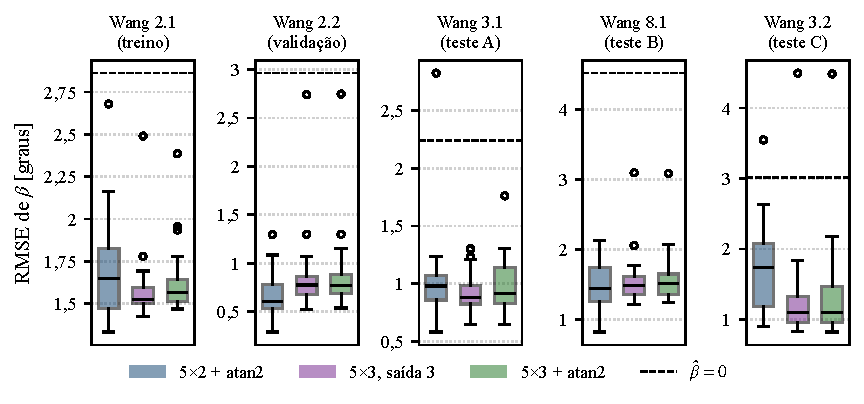
\includegraphics[width=\textwidth]{figuras/rmse_beta_boxplot.pdf}
    \fonte{Elaboração própria.}
\end{figure}

\begin{table}[htbp]
    \centering
    \caption{RMSE de $\beta$ (graus) por pista e variante: mediana, intervalo interquartil, média e desvio-padrão entre os modelos.}
    \label{tab:resumo_beta}
    \footnotesize
    \begin{tabular}{llrcccc}
        \toprule
        \textbf{Pista} & \textbf{Variante} & $n$ & \textbf{Mediana} & \textbf{[Q1; Q3]} & \textbf{Média} & \textbf{DP} \\
        \midrule
        Wang 2.1 (treino) & 5×2 + atan2 & 29 & 1,647 & [1,469; 1,825] & 1,683 & 0,300 \\
         & 5×3, saída 3 & 27 & 1,527 & [1,499; 1,593] & 1,582 & 0,197 \\
         & 5×3 + atan2 & 27 & 1,564 & [1,512; 1,641] & 1,626 & 0,200 \\
        Wang 2.2 (validação) & 5×2 + atan2 & 30 & 0,609 & [0,531; 0,784] & 0,665 & 0,216 \\
         & 5×3, saída 3 & 28 & 0,776 & [0,679; 0,859] & 0,853 & 0,403 \\
         & 5×3 + atan2 & 28 & 0,766 & [0,684; 0,880] & 0,864 & 0,408 \\
        Wang 3.1 (teste A) & 5×2 + atan2 & 30 & 0,979 & [0,858; 1,070] & 1,012 & 0,385 \\
         & 5×3, saída 3 & 28 & 0,882 & [0,823; 0,983] & 0,928 & 0,180 \\
         & 5×3 + atan2 & 28 & 0,917 & [0,826; 1,143] & 0,990 & 0,246 \\
        Wang 8.1 (teste B) & 5×2 + atan2 & 30 & 1,434 & [1,253; 1,739] & 1,507 & 0,339 \\
         & 5×3, saída 3 & 28 & 1,482 & [1,357; 1,608] & 1,541 & 0,352 \\
         & 5×3 + atan2 & 28 & 1,506 & [1,356; 1,647] & 1,574 & 0,360 \\
        Wang 3.2 (teste C) & 5×2 + atan2 & 30 & 1,738 & [1,183; 2,076] & 1,758 & 0,603 \\
         & 5×3, saída 3 & 28 & 1,098 & [0,960; 1,324] & 1,274 & 0,679 \\
         & 5×3 + atan2 & 28 & 1,099 & [0,961; 1,460] & 1,350 & 0,718 \\
        \bottomrule
    \end{tabular}
    \fonte{Elaboração própria.}
\end{table}


\begin{table}[htbp]
    \centering
    \caption{Testes confirmatórios nas pistas de teste: diferença de medianas com IC95\% \textit{bootstrap}, tamanho de efeito e valor-p corrigido por Holm em cada família.}
    \label{tab:testes}
    \scriptsize
    \begin{tabular}{lllcccrc}
        \toprule
        \textbf{Q} & \textbf{Comparação} & \textbf{Pista} & $n_1/n_2$ & \textbf{Dif.} & \textbf{IC95\%} & \textbf{Efeito} & \textbf{p (Holm)} \\
        \midrule
        Q1 & $\beta$: 5×3 atan2 $-$ 5×2 & Wang 3.1 & 28/30 & $-$0,062 & [$-$0,175; 0,128] & $-$0,00 & 1,0000 \\
        Q1 & $\beta$: 5×3 atan2 $-$ 5×2 & Wang 8.1 & 28/30 & 0,072 & [$-$0,158; 0,217] & 0,10 & 1,0000 \\
        Q1 & $\beta$: 5×3 atan2 $-$ 5×2 & Wang 3.2 & 28/30 & $-$0,639 & [$-$0,904; $-$0,291] & $-$0,50 & 0,0056 \\
        Q1 & $\beta$: 5×3 saída 3 $-$ 5×2 & Wang 3.1 & 28/30 & $-$0,097 & [$-$0,199; 0,026] & $-$0,15 & 1,0000 \\
        Q1 & $\beta$: 5×3 saída 3 $-$ 5×2 & Wang 8.1 & 28/30 & 0,048 & [$-$0,171; 0,168] & 0,06 & 1,0000 \\
        Q1 & $\beta$: 5×3 saída 3 $-$ 5×2 & Wang 3.2 & 28/30 & $-$0,641 & [$-$0,903; $-$0,362] & $-$0,59 & 0,0007 \\
        Q2 & $v_x$: 5×3 $-$ 5×2 & Wang 3.1 & 28/30 & 0,028 & [$-$0,087; 0,150] & 0,11 & 0,4887 \\
        Q2 & $v_x$: 5×3 $-$ 5×2 & Wang 8.1 & 28/30 & 0,093 & [0,026; 0,219] & 0,59 & 0,0006 \\
        Q2 & $v_x$: 5×3 $-$ 5×2 & Wang 3.2 & 28/30 & 0,256 & [0,137; 0,295] & 0,84 & $<$0,0001 \\
        Q2 & $v_y$: 5×3 $-$ 5×2 & Wang 3.1 & 28/30 & 0,033 & [$-$0,007; 0,062] & 0,34 & 0,1022 \\
        Q2 & $v_y$: 5×3 $-$ 5×2 & Wang 8.1 & 28/30 & 0,022 & [$-$0,035; 0,070] & 0,18 & 0,4678 \\
        Q2 & $v_y$: 5×3 $-$ 5×2 & Wang 3.2 & 28/30 & $-$0,068 & [$-$0,121; $-$0,020] & $-$0,24 & 0,3647 \\
        Q3 & $\beta$: saída 3 $-$ atan2 (5×3) & Wang 3.1 & 28/28 & $-$0,004 & [$-$0,020; $-$0,002] & 0,89 & 0,0002 \\
        Q3 & $\beta$: saída 3 $-$ atan2 (5×3) & Wang 8.1 & 28/28 & $-$0,017 & [$-$0,027; $-$0,007] & 0,71 & 0,1128 \\
        Q3 & $\beta$: saída 3 $-$ atan2 (5×3) & Wang 3.2 & 28/28 & $-$0,002 & [$-$0,009; 0,001] & 0,68 & 0,2545 \\
        \bottomrule
    \end{tabular}
    \par\footnotesize Nota: Q1 e Q2: Mann--Whitney, efeito = $\delta$ de Cliff (negativo: o 5×3 erra menos). Q3: Wilcoxon pareado por modelo, diferença = mediana das diferenças, efeito = fração de modelos em que a saída 3 erra menos. RMSE de $\beta$ em graus; de $v_x$, $v_y$ em m/s.
    \fonte{Elaboração própria.}
\end{table}


Em duas das três pistas de teste, Wang 3.1 e Wang 8.1, não há diferença significativa entre o ângulo obtido pelos modelos 5×3 (pela saída evoluída ou pelo $\operatorname{atan2}$ das velocidades) e o ângulo pós-calculado dos modelos 5×2. As diferenças de medianas ficam abaixo de 0,1° e os intervalos de confiança de 95\% incluem o zero, indo de cerca de $-0{,}2^\circ$ a $+0{,}2^\circ$. Os dados, portanto, não indicam diferença, mas também não permitem excluir diferenças dessa ordem, que correspondem a 15 a 20\% do RMSE mediano.

Na Wang 3.2, ao contrário, os modelos 5×3 erram menos: a mediana do RMSE cai de 1,74° para 1,10°, com $\delta$ de Cliff de $-0{,}59$ (efeito grande) e $p = 0{,}0007$ após a correção de Holm. Esse resultado vem de uma única pista e deve ser lido com cautela. Como descrito na \autoref{sec:proveniencia}, a velocidade lateral de referência das três pistas de teste está deslocada em relação ao valor implícito no ângulo de deriva bruto, o que pode favorecer ou prejudicar um braço conforme o viés de cada modelo.

Para medir essa sensibilidade, os modelos já treinados foram reavaliados, sem retreinamento, contra uma referência em que o deslocamento de $v_y$ (0,31, 0,37 e 0,31~m/s nas três pistas de teste) é subtraído antes do cálculo de $\beta$ (\autoref{tab:reavaliacao}). A comparação se inverte: com a referência corrigida, os modelos 5×2 erram menos do que os 5×3 nas três pistas. Para a saída evoluída, a diferença de medianas (5×3 menos 5×2) é de $+0{,}16^\circ$ na Wang 3.1, $+0{,}45^\circ$ na Wang 8.1 e $+0{,}28^\circ$ na Wang 3.2, com $\delta$ de Cliff de cerca de $+0{,}55$ e $p \le 0{,}002$ após a correção de Holm sobre as seis comparações. O viés, que era negativo para todos os estimadores em relação à referência original (entre $-0{,}6^\circ$ e $-1{,}4^\circ$), torna-se positivo em relação à corrigida (entre $+0{,}2^\circ$ e $+0{,}9^\circ$): os modelos ficam entre as duas referências. Removendo o viés, o RMSE contra a referência original é menor para o 5×3 na Wang 3.2 (0,77° contra 0,99°), praticamente igual na Wang 3.1 (0,65° contra 0,67°) e maior na Wang 8.1 (1,23° contra 0,82°); contra a referência corrigida, o 5×2 é melhor nas três. Portanto, a vantagem do 5×3 na Wang 3.2 não resiste à troca de referência, e os dados não permitem dizer qual das duas é a correta.

\begin{table}[htbp]
    \centering
    \caption{RMSE de $\beta$ (graus) nas pistas de teste, mediana entre modelos, contra a referência original e contra a referência com o deslocamento de $v_y$ removido; com e sem o viés.}
    \label{tab:reavaliacao}
    \small
    \begin{tabular}{llcccc}
        \toprule
        \textbf{Pista} & \textbf{Variante} & \multicolumn{2}{c}{\textbf{Referência original}} & \multicolumn{2}{c}{\textbf{Referência corrigida}} \\ & & RMSE & RMSE sem viés & RMSE & RMSE sem viés \\
        \midrule
        Wang 3.1 (teste A) & 5×2 + atan2 & 0,979 & 0,673 & 0,909 & 0,683 \\
         & 5×3, saída 3 & 0,882 & 0,645 & 1,071 & 0,861 \\
         & 5×3 + atan2 & 0,917 & 0,671 & 1,054 & 0,843 \\
        Wang 8.1 (teste B) & 5×2 + atan2 & 1,434 & 0,815 & 1,093 & 0,924 \\
         & 5×3, saída 3 & 1,482 & 1,233 & 1,539 & 1,283 \\
         & 5×3 + atan2 & 1,506 & 1,272 & 1,532 & 1,297 \\
        Wang 3.2 (teste C) & 5×2 + atan2 & 1,738 & 0,991 & 0,830 & 0,565 \\
         & 5×3, saída 3 & 1,098 & 0,773 & 1,108 & 0,697 \\
         & 5×3 + atan2 & 1,099 & 0,773 & 1,082 & 0,687 \\
        \bottomrule
    \end{tabular}
    \par\footnotesize Nota: deslocamentos de $v_y$ removidos: 0,31~m/s (Wang 3.1), 0,37~m/s (Wang 8.1) e 0,31~m/s (Wang 3.2).
    \fonte{Elaboração própria.}
\end{table}


Nas pistas exploratórias, o quadro é misto. Na Wang 2.2, os modelos 5×2 têm menor mediana (0,609° contra 0,776°); na pista de treino, os modelos 5×3 têm menor mediana (1,527° contra 1,647°) e menor dispersão. O critério de aprovação (RMSE finito, positivo e menor que 100) elimina apenas modelos divergentes e, portanto, introduz pouca seleção na Wang 2.2; a pista foi mantida como exploratória por ter participado desse critério. O resultado nela vai contra a ideia de que o 5×3 é sistematicamente melhor.

Considerando as cinco pistas, a mediana do RMSE de $\beta$ da saída evoluída é menor que a do 5×2 em três (Wang 2.1, 3.1 e 3.2) e maior em duas (Wang 2.2 e 8.1). Entre elas, apenas a diferença da Wang 3.2 é significativa nos testes confirmatórios.

A \autoref{tab:resumo_beta} mostra ainda que, em todas as pistas de teste, o intervalo interquartil do RMSE de $\beta$ é menor para a saída evoluída do que para o ângulo pós-calculado dos modelos 5×2 (na Wang 8.1, por exemplo, 0,25° contra 0,49°). O desvio-padrão, sensível a poucos modelos ruins, não acompanha esse padrão nas pistas Wang 8.1 e Wang 3.2, e a homogeneidade entre execuções não foi objeto de teste do plano de análise. Trata-se, portanto, de uma observação descritiva.

Na \autoref{tab:testes}, alguns intervalos de confiança excluem o zero enquanto o valor-p corrigido não é significativo (Q3 na Wang 8.1; $v_y$ na Wang 3.2). Isso pode ocorrer porque o intervalo é obtido por \textit{bootstrap} da diferença de medianas (ou da mediana das diferenças), enquanto o valor-p vem de um teste de postos corrigido por Holm; as duas medidas respondem a perguntas diferentes e a correção para múltiplas comparações reduz o poder.

\section{Efeito sobre as velocidades}\label{sec:q2}

A \autoref{fig:rmse_vel} e a \autoref{tab:resumo_vel} mostram o efeito da terceira saída sobre as estimativas de velocidade.

\begin{figure}[htbp]
    \centering
    \caption{Distribuição do RMSE de $v_x$ e de $v_y$ entre os modelos, por pista e por braço.}
    \label{fig:rmse_vel}
    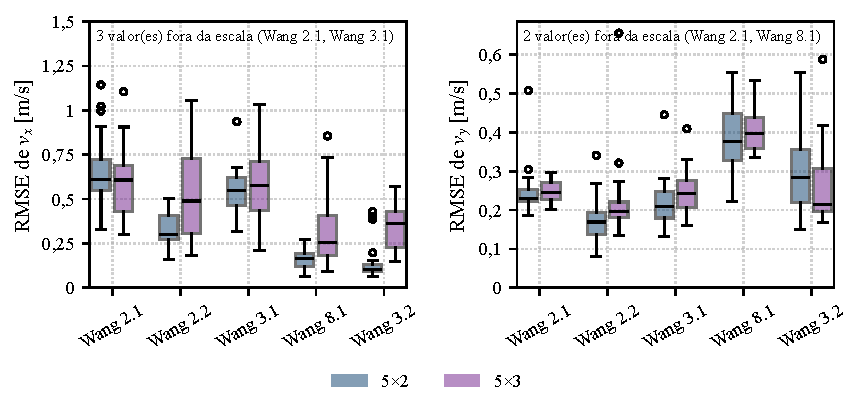
\includegraphics[width=\textwidth]{figuras/rmse_vxvy_boxplot.pdf}
    \fonte{Elaboração própria.}
\end{figure}

\begin{table}[htbp]
    \centering
    \caption{RMSE de $v_x$ e $v_y$ (m/s) por pista e braço: mediana e intervalo interquartil entre os modelos.}
    \label{tab:resumo_vel}
    \footnotesize
    \begin{tabular}{llrcccc}
        \toprule
        \textbf{Pista} & \textbf{Braço} & $n$ & \multicolumn{2}{c}{$v_x$} & \multicolumn{2}{c}{$v_y$} \\
        \midrule
        Wang 2.1 (treino) & 5×2 & 29 & 0,610 & [0,547; 0,723] & 0,231 & [0,221; 0,253] \\
         & 5×3 & 27 & 0,607 & [0,430; 0,690] & 0,245 & [0,226; 0,270] \\
        Wang 2.2 (validação) & 5×2 & 30 & 0,299 & [0,272; 0,405] & 0,169 & [0,138; 0,194] \\
         & 5×3 & 28 & 0,489 & [0,306; 0,729] & 0,195 & [0,180; 0,221] \\
        Wang 3.1 (teste A) & 5×2 & 30 & 0,550 & [0,465; 0,623] & 0,209 & [0,180; 0,248] \\
         & 5×3 & 28 & 0,579 & [0,434; 0,712] & 0,242 & [0,207; 0,277] \\
        Wang 8.1 (teste B) & 5×2 & 30 & 0,162 & [0,121; 0,191] & 0,376 & [0,327; 0,448] \\
         & 5×3 & 28 & 0,255 & [0,180; 0,405] & 0,397 & [0,358; 0,439] \\
        Wang 3.2 (teste C) & 5×2 & 30 & 0,104 & [0,092; 0,130] & 0,283 & [0,219; 0,356] \\
         & 5×3 & 28 & 0,359 & [0,228; 0,428] & 0,215 & [0,196; 0,307] \\
        \bottomrule
    \end{tabular}
    \fonte{Elaboração própria.}
\end{table}


A inclusão de $\beta$ piora a estimativa de $v_x$: nas pistas Wang 8.1 e Wang 3.2, a mediana do RMSE de $v_x$ passa de 0,16 para 0,26~m/s e de 0,10 para 0,36~m/s, respectivamente, com efeitos grandes ($\delta = 0{,}59$ e $0{,}84$) e significativos. Na estimativa de $v_y$, nenhuma diferença é significativa após a correção; a tendência é de leve piora na Wang 3.1 e de leve melhora na Wang 3.2. Esse resultado é coerente com a forma como o MGGP distribui o esforço: com a aptidão definida como a média simples dos três RMSE, e com o erro de $\beta$ em graus da mesma ordem dos erros das velocidades em m/s, o terceiro objetivo disputa com $v_x$ e $v_y$ o mesmo número de gerações e uma estrutura de indivíduo mais complexa.

\section{Saída evoluída e ângulo pós-calculado}\label{sec:q3}

Dentro de um mesmo modelo 5×3, a saída evoluída de $\beta$ e o ângulo calculado a partir das velocidades do próprio modelo são praticamente equivalentes. A mediana das diferenças vai de 0,002° a 0,017° (\autoref{tab:testes}); a saída evoluída é ligeiramente melhor na maioria dos modelos --- em 89\% deles na Wang 3.1, onde a diferença é significativa ---, mas a diferença é desprezível na prática. Isso sugere que a diferença observada na Wang 3.2 não vem de a saída $\beta$ ser mais precisa do que as velocidades do mesmo modelo, mas de os modelos 5×3 serem diferentes dos 5×2. Como a diferença em $v_y$ não foi significativa (\autoref{tab:testes}), o mecanismo dessa diferença não pôde ser identificado com os dados disponíveis.

\section{Erro por regime e simulação livre}\label{sec:regime}

Agrupando as pistas de teste, o RMSE de $\beta$ foi calculado por quartil de $|\beta|$ e de $v_x$ de cada pista (\autoref{tab:regime}). Por $|\beta|$, a variante A apresenta erro mediano entre 1,15° e 1,39°, e a saída evoluída do 5×3, entre 1,04° e 1,15°, sem tendência clara entre os quartis. Por $v_x$, o comportamento se inverte: no quartil de menor velocidade, a saída evoluída tem erro mediano de 1,03°, contra 1,37° da variante A; no quartil de maior velocidade, a variante A é melhor (0,68° contra 0,87°). O resultado é compatível com a \autoref{sec:angulo_deriva}: o $\operatorname{atan2}$ das velocidades estimadas amplifica o erro de $\hat v_y$ quando $v_x$ é baixo, e a saída evoluída, que não divide por $v_x$, é menos sensível a esse regime. A variante B\textsubscript{atan2} fica entre as duas, o que sugere que parte do ganho do 5×3 em baixa velocidade vem da forma como esses modelos estimam a própria $v_y$.

\begin{table}[htbp]
    \centering
    \caption{RMSE de $\beta$ (graus) por quartil de $|\beta|$ e de $v_x$ de cada pista: mediana entre modelos e pistas de teste.}
    \label{tab:regime}
    \small
    \begin{tabular}{llccc}
        \toprule
        \textbf{Eixo} & \textbf{Quartil} & \textbf{5×2 + atan2} & \textbf{5×3, saída 3} & \textbf{5×3 + atan2} \\
        \midrule
        $|\beta|$ & Q1 & 1,326 & 1,105 & 1,127 \\
         & Q2 & 1,149 & 1,041 & 1,051 \\
         & Q3 & 1,285 & 1,149 & 1,156 \\
         & Q4 & 1,394 & 1,056 & 1,113 \\
        $v_x$ & Q1 & 1,370 & 1,026 & 1,141 \\
         & Q2 & 1,236 & 1,117 & 1,203 \\
         & Q3 & 1,059 & 1,174 & 1,192 \\
         & Q4 & 0,676 & 0,866 & 0,901 \\
        \bottomrule
    \end{tabular}
    \par\footnotesize Nota: os quartis são os da própria pista (Q1 = menores valores); resultados descritivos, fora do plano de análise.
    \fonte{Elaboração própria.}
\end{table}


A \autoref{fig:sobreposicao} mostra a simulação livre de $\beta$ na pista de teste mais difícil para a variante A (Wang 3.2), para os modelos de RMSE mediano de cada braço. Os dois modelos acompanham as manobras --- inclusive os picos de cerca de $-10^\circ$ ---, mas ambos acumulam um desvio negativo a partir de cerca de 20~s, maior no modelo 5×2. Esse desvio é o principal componente do erro nessa pista e é discutido na \autoref{sec:limitacoes}.

\begin{figure}[htbp]
    \centering
    \caption{Simulação livre de $\beta$ na pista Wang 3.2 pelos modelos de RMSE mediano de cada braço (acima) e erro de estimação, referência menos estimativa (abaixo).}
    \label{fig:sobreposicao}
    \includegraphics[width=\textwidth]{figuras/dados/sobreposicao_beta.pdf}
    \fonte{Elaboração própria com dados da Universidade de Jilin.}
\end{figure}

\section{Estrutura das equações}\label{sec:estrutura}

As equações de $\beta$ dos 28 modelos 5×3 foram expandidas algebricamente, e os coeficientes dos monômios lineares de cada variável foram somados (\autoref{tab:estrutura_beta}).

\begin{table}[htbp]
    \centering
    \caption{Estrutura da equação de $\beta$ nos modelos 5×3: soma dos coeficientes dos monômios lineares de cada variável (qualquer atraso) após a expansão algébrica dos genes.}
    \label{tab:estrutura_beta}
    \footnotesize
    \begin{tabular}{p{7.2cm}cc}
        \toprule
        \textbf{Grandeza} & \textbf{Mediana [Q1; Q3]} & \textbf{Modelos} \\
        \midrule
        $\sum\theta$ persistência $\beta$ (esperado $\approx$ 1) & 0,9995 [0,9993; 0,9996] & 28 \\
        $\sum\theta$ $a_y$ (deg/(m/s²); cinemática $\approx$ 0.2865/$v_x$) & 0,01043 [0,009595; 0,0115] & 27 \\
        $\sum\theta$ $\dot\psi$ (deg/(rad/s); cinemática $\pm$0.2865) & 0 [0; 0] & 8 \\
        $\sum\theta$ $v_y$ (deg/(m/s)) & 0 [0; 0] & 7 \\
        maior $|\theta|$ de um atraso de $v_y$ & 0 [0; 4,352e-05] & 7 \\
        $\sum|\theta|$ não lineares & 0,004417 [0,003751; 0,00621] & 27 \\
        \bottomrule
    \end{tabular}
    \fonte{Elaboração própria.}
\end{table}


A soma dos coeficientes de monômios com escalas diferentes não mede a contribuição de cada termo ao erro, porque o peso de um termo depende também da magnitude do seu regressor. A \autoref{tab:estrutura_beta} indica, portanto, a presença de cada estrutura nas equações, e não a sua importância relativa.

Todas as equações contêm um termo de persistência em $\beta$, com soma de coeficientes de 0,9995 (mediana), e 27 das 28 contêm termos lineares em $a_y$, cuja soma de coeficientes tem mediana de 0,0104 graus por m/s². Comparando com a \autoref{eq:beta_cinematica} discretizada, em graus, $\beta[k] = \beta[k-1] + T\,\frac{180}{\pi}\,\big(a_y/v_x - \dot\psi\big)$, o coeficiente de $a_y$ deveria ser $0{,}2865/v_x$; o valor encontrado corresponde a uma velocidade de cerca de 27~m/s, acima da velocidade típica dos ensaios, o que indica que o termo linear em $a_y$ é apenas parte da correção. Como não há operador de divisão, o algoritmo não pode representar $a_y/v_x$ exatamente e aproxima a razão por um coeficiente constante, corrigido por termos não lineares de menor peso, presentes em 27 modelos. Os modelos recuperam, para $\beta$, parte da estrutura cinemática: um termo de persistência com soma de coeficientes próxima de 1 (comportamento de integrador, com um pequeno vazamento que impede o acúmulo ilimitado de erro) e um termo linear em $a_y$. O termo linear em $\dot\psi$ aparece em apenas 8 dos 28 modelos, de modo que a estrutura da \autoref{eq:beta_cinematica} é recuperada apenas parcialmente. A hipótese de que o acoplamento com a guinada apareça em produtos com outras variáveis não foi verificada. O modelo linear com os mesmos regressores e sem realimentação das saídas tem RMSE de $\beta$ bem maior (\autoref{tab:linear}), e o linear com realimentação divergiu; isso indica que um modelo linear simples com esses atrasos não reproduz o desempenho dos modelos MGGP, mas não permite isolar a contribuição dos termos não lineares dessa estrutura de integração. Um exemplo de equação de $\beta$ de um modelo 5×3, expandida e simplificada, é apresentado no Apêndice~A.

A inspeção mostra também como a terceira saída altera as demais equações. Nas equações de $v_y$ dos modelos 5×3, 93\% contêm termos com outra saída realimentada (inclusive $\beta$), contra 40\% nas equações de $v_y$ dos modelos 5×2. A terceira saída, portanto, não é apenas um subproduto: ela passa a fazer parte da estrutura que estima $v_y$, o que explica por que as velocidades dos modelos 5×3 diferem das dos 5×2 (\autoref{sec:q2}). Os modelos 5×3 são também maiores, com cerca de 102 nós por modelo (mediana) contra 69 dos 5×2, sem correlação relevante entre tamanho e erro de $\beta$ nas pistas de teste.

\section{Limitações}\label{sec:limitacoes}

Os resultados devem ser lidos à luz das seguintes limitações:

\begin{alineas}
    \item referência nas pistas de teste: nas três pistas de teste, a velocidade lateral de referência carrega um deslocamento constante de $+0{,}30$ a $+0{,}37$~m/s em relação ao valor implícito no ângulo de deriva bruto (\autoref{sec:proveniencia}), ausente na pista de treino. Um deslocamento $\delta$ em $v_y$ desloca $\beta$ em aproximadamente $\delta/v_x$, ou cerca de 1° a 15~m/s. Todos os estimadores apresentam viés negativo nessas pistas (medianas entre $-0{,}6^\circ$ e $-1{,}4^\circ$), compatível com esse efeito; parte do erro reportado, portanto, não é do estimador, mas da referência. A reavaliação com o deslocamento removido (\autoref{sec:q1}) inverte a comparação entre braços nas três pistas e torna o viés positivo, de modo que o resultado depende da referência adotada, e não foi possível determinar qual delas está correta;
    \item uma única base de dados e uma única configuração: todos os modelos foram treinados no mesmo ensaio, com a configuração T48, escolhida na IC por ter o melhor desempenho em modelos 5×2. Essa configuração pode favorecer o braço 5×2, e não se avaliou se o resultado se mantém com outras configurações, como a T19, ou com outros veículos;
    \item aptidão e unidade de $\beta$: a aptidão é a média simples dos RMSE das saídas, sem normalização. A inclusão da terceira saída reduz o peso de $v_x$ de 1/2 para 1/3, e $\beta$ foi treinado em graus. A piora de $v_x$ pode refletir, em parte, essas escolhas, e não foi feita análise de sensibilidade a elas;
    \item apenas modelos aprovados: a comparação usa os modelos aprovados na validação; 2 de 30 modelos 5×3 foram reprovados, contra nenhum 5×2 (\autoref{sec:campanha}). O braço 5×3 foi encerrado com 28 modelos, em vez dos 30 planejados; os testes usados não exigem grupos de mesmo tamanho;
    \item critério de divergência: um modelo 5×3 apresentou RMSE de $v_x$ de cerca de 1\,340~m/s na pista de treino sem ser classificado como divergente, pois suas estimativas ficaram abaixo do limiar de $10^4$. Esse valor afeta as médias da pista de treino, mas não as medianas nem os testes, que usam apenas as pistas de teste;
    \item número de pistas de teste: os valores-p refletem a variabilidade entre execuções independentes dentro de cada pista. Com três pistas, a variação entre cenários de condução não é capturada, e o ganho observado em uma das três pistas não pode ser generalizado;
    \item linha de base linear limitada e ausência de comparação com a literatura: o modelo linear com realimentação divergiu e o sem realimentação não é equivalente aos modelos MGGP; não foram avaliados modelos lineares ajustados por erro de simulação, nem estimadores da literatura com fusão sensorial. Assim, não se isolou o que os termos não lineares do MGGP acrescentam a uma estrutura de integração com vazamento;
    \item seleção da configuração: as pistas Wang 3.1 e Wang 8.1 participaram da escolha da configuração T48 na IC (\autoref{sec:base_dados}); apenas a Wang 3.2 é totalmente independente dessa escolha.
\end{alineas}

\chapter{CONCLUSÃO}\label{sec:conclusao}

Este trabalho comparou duas formas de obter o ângulo de deriva com o sensor virtual MGGP da IC: como terceira saída do modelo (28 modelos 5×3 aprovados) ou calculado a partir das velocidades estimadas (30 modelos 5×2), em simulação livre em três pistas de teste.

Quanto à primeira pergunta, a resposta depende da pista. Em duas das três pistas de teste não houve diferença significativa, e os intervalos de confiança não permitem excluir diferenças de até cerca de 0,2°. Na Wang 3.2, os modelos 5×3 reduziram a mediana do RMSE de $\beta$ de 1,74° para 1,10°, com efeito grande. Esse resultado vem de uma única pista e, nessa pista, como nas demais de teste, a velocidade lateral de referência está deslocada em cerca de 0,3~m/s em relação ao valor implícito no ângulo de deriva bruto, o que pode favorecer ou prejudicar um braço conforme o viés de cada modelo. De fato, a reavaliação com o deslocamento removido inverte a comparação: com a referência corrigida, os modelos 5×2 erram menos do que os 5×3 nas três pistas de teste (diferenças de medianas de $+0{,}16^\circ$ a $+0{,}45^\circ$). Como os dados não permitem dizer qual das referências está correta, o ganho do 5×3 na Wang 3.2 não pode ser tomado como evidência. Nas pistas exploratórias o resultado foi misto: o 5×2 teve menor mediana na Wang 2.2 e o 5×3 na pista de treino. Os modelos 5×3 tiveram menor intervalo interquartil nas pistas de teste e menor erro no quartil de menor velocidade (mediana de 1,03° contra 1,37°); no quartil de maior velocidade, porém, o ângulo pós-calculado dos modelos 5×2 foi melhor (0,68° contra 0,87°). Esses são resultados descritivos, fora do plano de análise.

Quanto à segunda pergunta, a terceira saída tem custo: a estimativa de $v_x$ piorou de forma significativa, com efeito grande, em duas das três pistas de teste; a de $v_y$ não se alterou de forma significativa; o custo de cada treinamento aumentou cerca de 70\%; e 2 dos 30 treinamentos 5×3 foram reprovados, contra nenhum dos 5×2.

Quanto à terceira pergunta, a saída evoluída e o ângulo calculado a partir das velocidades do próprio modelo 5×3 são praticamente equivalentes. Como a diferença em $v_y$ não foi significativa, o mecanismo do ganho observado na Wang 3.2 não foi identificado.

As equações de $\beta$ recuperam parcialmente a estrutura cinemática $\dot\beta \approx a_y/v_x - \dot\psi$: um termo de persistência próximo de 1 e um termo linear em $a_y$ aparecem na quase totalidade dos modelos, mas o termo linear em $\dot\psi$ aparece em apenas 8 dos 28. O estimador cinemático simples derivou na pista de treino, a mais longa e com trechos de baixa velocidade. Um modelo linear com os mesmos regressores e sem realimentação teve RMSE de $\beta$ de 1,8° a 4,0° nas pistas de teste, maior do que o dos modelos MGGP, e o linear com realimentação divergiu; ainda assim, não se separou a contribuição dos termos não lineares do MGGP.

Com a evidência disponível, não é possível afirmar que a terceira saída melhora o ângulo de deriva de forma geral. Se o ângulo de deriva é a única grandeza de interesse e o custo adicional é aceitável, o modelo 5×3 só é uma opção se a referência original estiver correta, pois com a referência corrigida o 5×2 foi melhor; se as velocidades também são usadas, o modelo 5×2 com $\beta$ pós-calculado preserva a qualidade de $v_x$ com menor custo de treinamento.

As principais limitações, discutidas na \autoref{sec:limitacoes}, são a base de dados e a configuração únicas, o deslocamento da velocidade lateral de referência nas pistas de teste e o número reduzido de pistas. Como trabalhos futuros, sugere-se: (i) esclarecer a origem desse deslocamento, com a equipe que coletou os dados, para definir qual referência é a correta; (ii) incluir uma linha de base linear com realimentação estável, por exemplo ajustada por erro de simulação; (iii) avaliar a sensibilidade à unidade de $\beta$ e à normalização da aptidão; (iv) incluir o operador de divisão protegida, para que o MGGP represente diretamente $v_y/v_x$ e $a_y/v_x$; (v) repetir a comparação com a configuração T19, de menor custo, e com mais pistas e veículos; (vi) investigar a poda estrutural baseada no \textit{Forward-Regression Orthogonal Estimator} (FROE), que a IC não conseguiu usar com a arquitetura MIMO; e (vii) combinar o estimador cinemático com o sensor virtual, usando o MGGP apenas para corrigir a deriva da integração.


%==============================================================================
% Bibliografia

% Carrega o estilo para referências ABNT
\bibliographystyle{abntex2-alf}            

% Alterando informações do estilo de citação.
% Como estamos usando uma versão alterada, essas opções são necessárias.
% Et al. em itálico
\citeoption{abnt-etal-text=it}

% Até 3 autores antes do et al.
\citeoption{abnt-etal-cite=3}

% Colocar s.d. na falta de um ano de publicação
\citeoption{abnt-missing-year=sd}

% Altera o estilo de citação para (Autor, ano)
% A opção abnt-cite-style=AuthorYEAR está quebrada; essa é equivalente.
\citeoption{abnt-nbr10520=1988} 


% Comando necessário para corrigir o título das referências.
% Para o estilo ABNT, esse comando SEMPRE deve ser
% chamado antes do \bibliography
\referencias
% Adiciona as referência em bibtex 
\bibliography{referencias}

%==============================================================================
% Outros elementos pós-textuais


% Anexos e apêndices
% Os anexos devem ser includios antes
% e utilizar \input ao invés de \include, para não criar uma nova página
% Anexos

% Apêndice A (esqueleto): equação de beta de um modelo 5x3 típico
\apendice{Equação de $\beta$ de um modelo 5×3 típico}\label{apen:equacao_beta}

Este apêndice apresenta a equação da terceira saída de um modelo 5×3 de RMSE mediano na pista Wang 3.2, o mesmo modelo da \autoref{fig:sobreposicao} (tentativa 12, semente 2038). O RMSE de $\beta$ desse modelo é de 2,49° na pista de treino, 0,86° na Wang 2.2, 0,83° na Wang 3.1, 1,51° na Wang 8.1 e 1,10° na Wang 3.2.

Os sete genes da saída 3 foram expandidos algebricamente, o que resulta em 16 monômios. Os monômios com coeficiente de módulo inferior a $10^{-4}$ (um termo em $a_y$ com atraso de 61 amostras e seis produtos de três variáveis) foram descartados, por não alterarem a saída de forma perceptível. Com $\beta$ em graus, $a_y$ em m/s², $\omega_r$ e $\dot\psi$ em rad/s, e $x[k-n]$ o valor de $x$ há $n$ amostras (200~Hz), a equação resultante é
\begin{align}
    \beta[k] \approx{}& 1{,}0113\,\beta[k-1] - 0{,}0045\,\beta[k-9] - 0{,}0027\,\beta[k-32] - 0{,}0045\,\beta[k-40] \nonumber\\
    &+ 0{,}0024\,a_y[k-1] + 0{,}0045\,a_y[k-3] + 0{,}0027\,a_y[k-6] \nonumber\\
    &+ 0{,}0032\,\dot\psi[k-1]\,\omega_r[k-1] - 0{,}0008.
    \label{eq:beta_modelo_tipico}
\end{align}

A soma dos coeficientes de $\beta$ é 0,9997, de modo que o modelo se comporta como um integrador com pequeno vazamento, como discutido na \autoref{sec:estrutura}. A soma dos coeficientes lineares de $a_y$ é 0,0095~graus por m/s², próxima da mediana de 0,0104 dos 28 modelos. O termo da taxa de guinada aparece apenas no produto $\dot\psi\,\omega_r$, e não como termo linear.





%==============================================================================
% Fim do documento
%==============================================================================
\end{document}
